\documentclass[11pt,a4paper]{article}
\usepackage[T1]{fontenc}
\usepackage{lmodern,microtype}
\usepackage{amsmath,amssymb,mathtools,mathrsfs}
\usepackage[margin=25mm]{geometry}
\usepackage{graphicx,booktabs,tabularx,array}
\usepackage[section]{placeins}
\usepackage{xcolor,xurl}
\usepackage[colorlinks=true,allcolors=blue]{hyperref}
\setlength{\parskip}{.35em}
\setlength{\parindent}{0pt}
\setlength{\emergencystretch}{2em}
\allowdisplaybreaks[2]
\hypersetup{pdftitle={Lorentzian Einstein-Cartan Reduction on Compact Homogeneous Geometries: Constraints and Inhomogeneous Perturbations},pdfauthor={Muacca},pdfsubject={Version 2, revised 2026-11-08}}
\title{Lorentzian Einstein--Cartan Reduction on Compact Homogeneous Geometries: Constraints and Inhomogeneous Perturbations}
\author{Muacca}\date{Version 2\\Revised: 2026-11-08\\First release: 2026-06-14}
\begin{document}\maketitle\begin{abstract}
We study inhomogeneous constraints in source-free Lorentzian Einstein--Cartan theory with constant complete Nieh--Yan coupling on fixed compact geometries. The regular homogeneous metric counts remain 5, 3, 2 and 2 pairs on the torus, Nil, Sol and the three-sphere, with symmetric-background exceptions treated separately. For nonzero flat-torus modes, connection-retaining and metric reductions agree in the action and reduced two-form. Under the stated compact CMC hypotheses, the Arms--Marsden--Moncrief theorem makes the four Taub conditions necessary and sufficient for local integrability; explicit standing-wave and nonparallel two-wave corrections satisfy the local vacuum equations through second order. On selected time-dependent curved vacuum backgrounds, we construct closed tensor blocks on LRS Nil, infinite dual-orbit systems on Sol, and low Wigner blocks on Taub, with gauges, canonical reductions and reconstruction. On the fixed Sol background, the no-KID theorem gives local integrability of all real full linearized constraint data in the stated Sobolev class, including admissible Gowdy and common-core dual-orbit data. Quadratic KID conditions on Nil and Taub remain necessary conditions only. Finite-time examples include an independent Lorenz evolution on one Sol orbit, with interior spatial, window and time convergence comparisons. Convergence in the reduced fourth-order form, whole-line numerical error bounds, general stability, nonlinear closure within a fixed sector and lifting sufficiency on Nil and Taub are not established.
\end{abstract}
\section{Question and results}

We study the passage from homogeneous constraints to inhomogeneous perturbations on fixed compact spaces in source-free Lorentzian Einstein--Cartan (EC) theory with constant complete Nieh--Yan (NY) coupling. Elimination of the independent connection, the linear gauge quotient, and tangency to an exact vacuum family are distinct stages of the same variational problem.

We use the action, quotient and boundary conventions of Papers01--05 \cite{paper1,paper2,paper3,paper3ec,paper4,paper5}. Paper06 treated the full equations of common-scale families, the homogeneous volume--shape cone and its exact homogeneous realization \cite{paper6}. Here these results provide the starting point for spatially dependent fields, closed harmonic blocks and background-dependent integral conditions.

First, the regular homogeneous metric strata have 5/3/2/2 canonical pairs on $T^3$/Nil/Sol/$S^3$. The static torus and symmetric Taub points are treated separately. For nonzero flat-torus modes, direct reduction before and after Lorentz gauge fixing and connection elimination gives the same quadratic dynamics and reduced two-form.

Second, the four flat-torus Taub conditions are necessary and sufficient for local integrability under the hypotheses of the Arms--Marsden--Moncrief theorem \cite{ArmsMarsdenMoncrief1982}. We give explicit second-order corrections for a standing wave with homogeneous expansion and retain all thirteen generated wavevectors for two nonparallel waves. The theorem application and the finite-order construction have different logical roles.

Third, we reduce inhomogeneous constraints on selected time-dependent vacuum backgrounds of Nil, Sol and $S^3$. We treat the central-zero and central-nonzero Nil sectors, fiber-independent Sol modes and general nonzero dual orbits, and four low Wigner labels on $S^3$, with complete reconstruction for $j=3/2$. Finite-time examples include an independent Lorenz evolution on Sol with interior convergence comparisons.

Two propagating field species, the total canonical pairs in a representation block, and the homogeneous regular-stratum count are different quantities. For Nil and Taub we establish quadratic necessary KID conditions. On the fixed Sol background, absence of KIDs and the existing theorem give local integrability of all full linearized constraint data in the stated Sobolev class (Section 7 and Appendix G). All-time stability and a complete physical spectrum are not established. Closed forms, finite metric paths and spatial Laplacians remain separate geometric data in Appendix E.

Auxiliary connection elimination, the two gravitational polarizations and linearization stability belong to established theory \cite{Hehl1976,Pons2010,BrillDeser1973,ArmsMarsdenMoncrief1982,FischerMarsdenMoncrief1980}. The concrete content here is the explicit constraints, reductions, reconstructions and second-order corrections for the stated action and quotients, with their counting units and domains.

%==============================================================================
% Section 2: Lorentzian EC+NY setup and Bianchi class-A backgrounds
%==============================================================================
\section{Lorentzian EC+NY setup and Bianchi class-A backgrounds}
\label{sec:setup}

\subsection{First-order action ingredients}
\label{sec:setup:action}

The basic variables are the tetrad one-form $e^{I}$ and the Lorentz connection
one-form $\omega^{IJ}$, both treated as independent (first-order / Palatini
type).  The action consists of the Einstein--Cartan term~\cite{ref8} and the
Nieh--Yan term~\cite{ref9}:
\begin{equation}
  S[e,\omega]
  =\frac{1}{2\kap^{2}}\int \epsilon_{IJKL}\, e^{I}\wedge e^{J}\wedge R^{KL}[\omega]
  +\frac{\thetaNY}{\kap^{2}}\int \left( T^{I}\wedge T_{I}
       - e_{I}\wedge e_{J}\wedge R^{IJ} \right),
\end{equation}
where $R^{IJ}[\omega]=\dd\omega^{IJ}+\omega^{I}{}_{K}\wedge\omega^{KJ}$ and
$T^{I}=\dd e^{I}+\omega^{I}{}_{J}\wedge e^{J}$.  The signature and the
Hodge/$\epsilon$ conventions are fixed in Appendix~\ref{app:conventions}.

\paragraph{Treatment of the NY term.}
We adopt the route that treats the NY term as an exact four-form (the NY-MAIN
route).  Within our NY-MAIN route and the inspected reduced/native-action gate
of the LZ-native $\AX/\VT/\MX$ torsion ansatz scalars, the NY term contributes
on the background only as an exact boundary term.  In the reduced system it
forms an exact auxiliary shell, and its promotion to fields $\eta(x),V(x)$
generates no quadratic kinetic/gradient term under the inspected native-action
criterion (Section~\ref{sec:torsion}).  The topological nature of the NY term in
the canonical analysis is known~\cite{ref33,ref34,ref35}.  This statement of
bulk non-involvement is restricted to the above scope and does not extend
automatically to a full torsion field theory or to a general NY action.

\subsection{Bianchi class-A backgrounds and the structure matrix}
\label{sec:setup:structure}

The spatial sections carry the left-invariant structure of a three-dimensional
unimodular Lie group $G$.  The left-invariant one-forms $\sigma^{i}$
($i=1,2,3$) satisfy
\begin{equation}
  \dd\sigma^{i}=-\tfrac12\,C^{i}{}_{jk}\,\sigma^{j}\wedge\sigma^{k}.
\end{equation}
The class-A (unimodular) condition is $C^{j}{}_{ij}=0$~\cite{ref15}, and then the
structure constants are encoded in a symmetric \emph{structure matrix}
$n^{ij}$:
\begin{equation}
  C^{i}{}_{jk}=\epsilon_{jkl}\,n^{li},
  \qquad
  n^{ij}=\tfrac12\,\epsilon^{ikl}\,C^{j}{}_{kl},
  \qquad n^{ij}=n^{ji}.
\end{equation}
By the Milnor frame~\cite{ref16}, $n^{ij}=\mathrm{diag}(n_{1},n_{2},n_{3})$, and
its rank/signature classifies the class-A type.  The four topologies treated
here are collected in Table~\ref{tab:bianchi}.  Bianchi models with compact
spatial sections are restricted to class A~\cite{ref19,ref20}.

\begin{table}[H]
\centering
\begingroup
\renewcommand{\arraystretch}{1.4}
\begin{tabular}{llcrrrr}
\toprule
Topology & Bianchi & $n$ (Milnor frame) & $\rank(n)$ & $\dzero=3-\rank(n)$ & $b_{1}$ & $R\,q^{2}$ \\
\midrule
$\Tthree$   & I    & $\mathrm{diag}(0,0,0)$  & 0 & 3 & 3 & $0$    \\
$\Nilthree$ & II   & $\mathrm{diag}(1,0,0)$  & 1 & 2 & 2 & $-1/2$ \\
$\Solthree$ & VI$_{0}$ & $\mathrm{diag}(1,-1,0)$ & 2 & 1 & 1 & $-2$   \\
$\Sthree$   & IX   & $\mathrm{diag}(1,1,1)$  & 3 & 0 & 0 & $6$    \\
\bottomrule
\end{tabular}
\endgroup
\caption{Four Bianchi class-A backgrounds.  Here $b_{1}$ is the first Betti
number of the corresponding compact quotient (standard values~\cite{ref18}), and
$R\,q^{2}$ is the dimensionless spatial scalar curvature at the isotropic point.}
\label{tab:bianchi}
\end{table}

The $\Sthree$ structure-constant normalisation is fixed to $C=\epsilon$ ($|C|=1$)
throughout (Appendix~\ref{app:conventions}, where the explicit conversion to the
normalisation of paper~VI~\cite{ref7} is also recorded).  The quantities
$\rank(n)$ and $\dzero$ are invariant under an overall structure-constant scaling
$C\to sC$, whereas the \emph{numerical} values such as $R\,q^{2}$ and the TT
eigenvalues depend on $s$ (Appendix~\ref{app:conventions:s3}).

The $\dzero$ in Table~\ref{tab:bianchi} is the algebraic prediction from the
rank defect of the structure matrix.  That this is realised as the kernel of the
constrained spectrum is the main result of this paper
(Section~\ref{sec:rankdefect}).  The relation to abelianisation,
$\dim(\mathfrak{g}/[\mathfrak{g},\mathfrak{g}])=\dim\ker n$, is also a known
algebraic fact and is used only as a geometric cross-check.

\subsection{Background ansatz and perturbation sectors}
\label{sec:setup:perturbation}

The background is taken as the homogeneous diagonal ansatz
\begin{equation}
  e^{0}=N(t)\,\dd t,\qquad
  e^{a}=q_{a}(t)\,\sigma^{a} \quad (a=1,2,3;\ \text{no sum}),
\end{equation}
and the connection $\omega^{IJ}$ has independent homogeneous components (the
explicit component list and the reduced action are in
Appendix~\ref{app:native}).  Relative to the background frame the perturbations
decompose into

\begin{itemize}
  \item a \textbf{scalar (diagonal/axis) sector}: diagonal metric perturbations
        $\beta_{a}$ and the corresponding connection perturbations,
  \item a \textbf{spin-1 (transverse vector) sector},
  \item a \textbf{spin-2 (TT) sector}: transverse-traceless perturbations
        $h^{\mathrm{TT}}_{ab}$.
\end{itemize}

The analysis of the homogeneous modes ($k=0$) is central to
Section~\ref{sec:rankdefect}, while the inhomogeneous modes are treated by a
topology-dependent harmonic expansion ($\Tthree$: Fourier; $\Sthree$:
hyperspherical harmonics~\cite{ref28,ref29}; $\Nilthree$: toroidal $\cup$
Heisenberg sector; $\Solthree$: boost sector) in Section~\ref{sec:spectral} and
Appendix~\ref{app:spectral}.

\subsection{Torsion ansatz scalars}
\label{sec:setup:torsion}

On the homogeneous background, the torsion within the ansatz used here organises
into the following scalar modes:

\begin{itemize}
  \item \textbf{AX (axial)}: an axial scalar $\eta(t)$ giving
        $T^{a}{}_{bc}\supset\eta\,\epsilon_{abc}$;
  \item \textbf{VT (vector/trace)}: a scalar $V(t)$ giving the trace part;
  \item \textbf{MX (mixed)}: the mixed branch of the two.
\end{itemize}

These are the same family as the branch classification (EH/AX/VT/MX) of
papers~V/VI~\cite{ref6,ref7}.  Section~\ref{sec:torsion} classifies the
derivative couplings obtained when these are promoted to fields
$\eta(x),V(x)$.  All torsion claims of this paper lie \emph{within the
$\AX/\VT/\MX$ ansatz scalars}; no generalisation to a full 24-component torsion
field theory is claimed.

\subsection{Notation summary}
\label{sec:setup:notation}

In what follows, $q^{2}$ denotes the square of the isotropic scale factor (the
isotropic point $q_{1}=q_{2}=q_{3}=q$), $\kap^{2}=8\pi G$, and $\vol$ denotes
the comoving volume of the spatial cell.  The notation of the constraint
analysis (primary/secondary constraints, first/second class, Dirac bracket)
follows the standard definitions~\cite{ref10,ref11,ref12}.

%==============================================================================
% Section 3: DBR reduction protocol and route justification
%==============================================================================
\section{DBR reduction protocol and route justification}
\label{sec:dbr}

\subsection{The Dirac-before-Routh protocol}
\label{sec:dbr:protocol}

The phase space of the first-order EC+NY system consists of the tetrad, the
connection, and their conjugate momenta, and it carries many primary
constraints.  Our reduction procedure adopts the following order \emph{as a
protocol}.

\begin{quote}
\textbf{DBR (Dirac-before-Routh) protocol.}
(i) Complete the Dirac--Bergmann algorithm~\cite{ref10,ref11,ref12}: generate
the secondary constraints from the consistency of the primary constraints, and
after closure classify first/second class and construct the Dirac bracket for
the second-class pairs.  (ii) Only then perform the Routh-type elimination /
reduction of the auxiliary variables (such as the non-dynamical connection
components) and present the reduced spectrum.
\end{quote}

DBR is not a new principle; it is the standard procedure of constrained
dynamics applied faithfully to this system.  The reverse order -- solving the
auxiliary connection variables by their field equations and substituting into
the action before the constraint analysis -- is called the \textbf{RBD
(Routh-before-Dirac)} route here.

\subsection{Why the order matters: a recognised issue}
\label{sec:dbr:order}

That substitution at the level of the action is not, in general, interchangeable
with substitution at the level of the equations of motion is an established
generality~\cite{ref13}.  Substitution is safe only for auxiliary variables
(whose own equations are algebraically solvable and free of derivatives);
otherwise a proof of equivalence is required.  In the Bianchi context it is also
classically known that the validity of imposing the symmetry at the level of the
action is restricted to class A (in class B it gives the wrong field
equations)~\cite{ref21,ref22}, and the equivalence of the Palatini and metric
formulations itself is a nontrivial statement to be proved by constraint
analysis~\cite{ref23}.  In adopting DBR as the standard, we select the order of
operations for which constraint equivalence is guaranteed against this known
``Palatini reduction non-commutativity'' (route dependence).

\subsection{Control experiment}
\label{sec:dbr:control}

To support the adoption of DBR empirically, we ran the RBD route as a
\textbf{control experiment}.  The verification was carried out in the Branch-A
scalar sector of the $\Sthree$ background.  The result is the following.

\begin{quote}
In the verified $\Sthree$ Branch-A scalar sector, eliminating the auxiliary
connection variables before the Dirac closure produces a Dirac-inequivalent
extra scalar mode.  The recomputation gives $N_{\rm phys}=0$ for
DBR\_KEEP\_ALL at all representative harmonic levels, whereas the spatial-$\omega$
and full-$K$ Routh variants give $N_{\rm phys}=1/1/2$ for $l=0,1,\ge2$.  At the
lowest harmonic level the comparison starts from the same Branch-A local
first-order Lagrangian, and reproduces the discrepancy DBR:0 / RBD:1 together
with $H_{PP}=-3/8<0$.  For $l\ge1$ the RBD extra count is treated as a
route-level gauge-breaking artefact; the negative-sign diagnostic is claimed
only at $l=0$ (scope details in Appendix~\ref{app:route}).
\end{quote}

This discrepancy is \emph{route-level}, not a physical instability.  We do not
draw from it any theorem that ``RBD is generally wrong.''  The claim is confined
to a single point: \emph{since route equivalence demonstrably fails in this
system, all subsequent physical topology claims are made within the DBR
protocol.}

\begin{table}[H]
\centering
\begingroup
\renewcommand{\arraystretch}{1.4}
\begin{tabularx}{\linewidth}{lLLl}
\toprule
Route & Order of closure and elimination & Outcome in $\Sthree$ Branch-A scalar sector & Status \\
\midrule
DBR & Dirac closure $\to$ Routh elimination &
$0$ physical scalars (kernel non-propagating; Section~\ref{sec:rankdefect}) &
\textbf{adopted} (standard) \\
RBD & Routh elimination $\to$ Dirac closure &
Dirac-inequivalent extra scalar mode ($H_{PP}=-3/8<0$ at $l=0$; route-level) &
control route (recorded) \\
\bottomrule
\end{tabularx}
\endgroup
\caption{Route taxonomy (compact version; details in
Appendix~\ref{app:route}).}
\label{tab:route}
\end{table}

\begin{figure}[H]
  \centering
  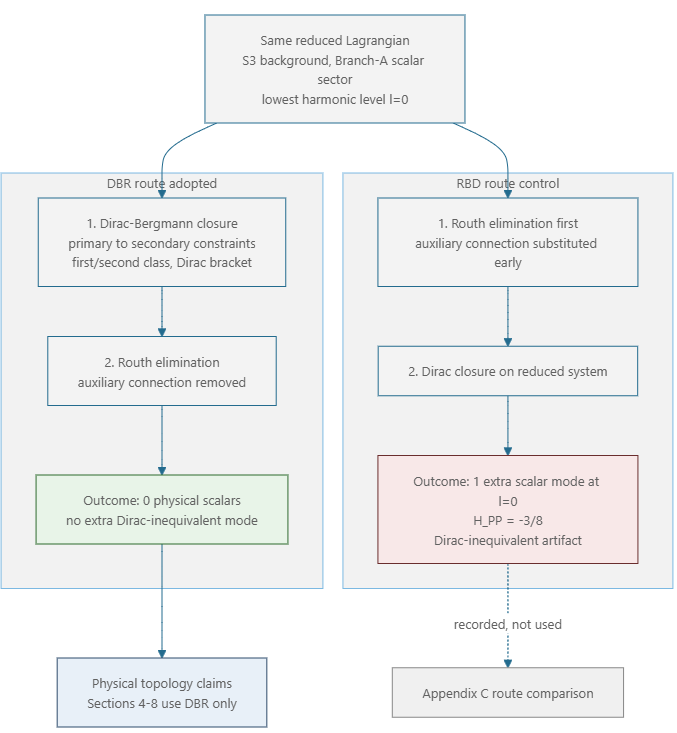
\includegraphics[width=0.95\textwidth]{figures/fig02_DBR-vs-RBD_route-comparison.png}
  \caption{DBR versus RBD route comparison.  From the same Branch-A local
    first-order Lagrangian, the two routes -- differing only in the order of
    operations -- are shown side by side.  DBR yields $0$ physical scalar
    degrees of freedom, while RBD gives a Dirac-inequivalent extra mode; at
    $l=0$ the diagnostic sign is $H_{PP}=-3/8<0$.  \emph{Scope}: the negative
    sign is claimed only for the lowest level; for $l\ge1$ the RBD extra count
    is recorded as a route-level gauge-breaking artefact.  The RBD outcome is
    not a physical instability.}
  \label{fig:route}
\end{figure}

\subsection{Scope declaration}
\label{sec:dbr:scope}

The claims of all subsequent sections
(Sections~\ref{sec:rankdefect}--\ref{sec:torsion}) are results under the DBR
protocol.  The RBD route is referred to only in the route-comparison details of
Appendix~\ref{app:route}.

\section{Connection elimination and constraint preservation}

We compare the connection-retaining and metric descriptions at the same perturbative order with the same action and endpoint data. The derivative-dependent LC substitution is not asserted to be a point canonical transformation on the unreduced space \cite{Pons2010}.

\stepcounter{equation}\begin{equation}\tag{D-01}\label{eq:D-01}
\frac{d\phi_A}{dt}=\{\phi_A,H_c\}+\{\phi_A,\phi_B\}\lambda^B\simeq0,\qquad H_T=H_c+\lambda^B\phi_B.
\end{equation}

In primary preservation, the image of the Poisson matrix fixes multipliers; only its left kernel produces new constraints. The original primary multipliers are retained at every consistency stage. Appendix C gives the scalar actions (D-02)--(D-03) and their closure.

\subsection{Direct comparison for a nonzero flat mode}

\begin{center}\small\begin{tabularx}{\textwidth}{@{}>{\raggedright\arraybackslash}X>{\raggedright\arraybackslash}X>{\raggedright\arraybackslash}X>{\raggedright\arraybackslash}X>{\raggedright\arraybackslash}X@{}}\toprule
Description & Configurations & First class & Second class & Pairs\\\midrule
Lorentz retained & 40 & 20 & 36 & 2\\
Lorentz fixed & 34 & 8 & 48 & 2\\
Metric & 10 & 8 & 0 & 2\\
\bottomrule\end{tabularx}\end{center}

The table is for one real Fourier quadrature. Retaining all 24 connection components and symbolic $k\ne0$, the reduced action, endpoint-derived two-form and the kinetic and gradient coefficients of both polarizations agree with (W-02) in all three descriptions. Including both real quadratures gives four real canonical pairs.

\stepcounter{equation}\begin{equation}\tag{D-05}\label{eq:D-05}
\Theta_{\rm ret}\big|_{\omega_{\rm LC}}-\Theta_{\rm met}=\delta B,
\qquad \Omega_{\rm ret}\big|_{\omega_{\rm LC}}-\Omega_{\rm met}=\delta^2B=0.
\end{equation}

$B$ includes the Lorentz total derivative and the complete NY endpoint. The current mixing the two real quadratures is retained, combining both NY terms from the same connection. For curved backgrounds we use the full Cartan solution, the auxiliary quadratic form and endpoint identities. We do not claim a new complete unreduced Dirac chain for every curved block; Appendix B specifies the directly verified scope.

\section{Regular homogeneous constraints and the static torus}

\stepcounter{equation}\begin{equation}\tag{H-03}\label{eq:H-03}
\begin{aligned}(A_k)^i{}_j&=n_{iz}\epsilon_{zkj},\qquad \mathcal L_\beta g=\beta^k(A_k^Tg+gA_k),\\ J_k&=\mathrm{tr}\bigl[\pi(A_k^Tg+gA_k)\bigr],\\ \{J_i,F\}&=0,\qquad \{J_i,J_j\}=-\epsilon_{ijk}n_kJ_k\quad(n=\mathrm{diag}(n_1,n_2,n_3)).\end{aligned}
\end{equation}

The symplectic form is $\Omega=\sum_{ij}\delta\pi^{ij}\wedge\delta g_{ij}$. After removing the lapse and shift primary multiplier pairs, $F$ and the independent $J_k$ generate first-class constraints. Internal Lorentz directions have already been quotiented in the metric description after solving torsion. Discrete quotient automorphisms are not subtracted as continuous gauge directions.

\stepcounter{equation}\begin{equation}\tag{H-04}\label{eq:H-04}
r=\mathrm{rank}\,dJ,\qquad \mathrm{rank}\,d(F,J)=r+1,\qquad N_{\rm hom}=6-r-1.
\end{equation}

Equation (H-04) is a local count on the regular open stratum of the constraint surface. Appendix C gives constraint-satisfying representatives and nonzero minors. The span of the $A_k$ bounds the number of independent $J_k$, and the representative minors attain that bound. Degenerate strata require a separate regularity check.

\begin{center}\small\begin{tabularx}{\textwidth}{@{}>{\raggedright\arraybackslash}X>{\raggedright\arraybackslash}X>{\raggedright\arraybackslash}X@{}}\toprule
Geometry & $\mathrm{rank}\,dJ$ & $\mathrm{rank}\,d(F,J)$\\\midrule
$T^3$ & 0 & 1\\
Nil & 2 & 3\\
Sol & 3 & 4\\
$S^3$ & 3 & 4\\
\bottomrule\end{tabularx}\end{center}

The counts $5/3/2/2$ concern the finite-dimensional system of all symmetric homogeneous metrics on the specified fixed quotients. They are not graviton polarizations per spacetime point, Teichm\"uller dimensions for arbitrary lattices, or zero-frequency counts at each background. Their objects and values differ from the $3/2/1/0$ closed-one-form dimensions.

\begin{figure}[htbp]\centering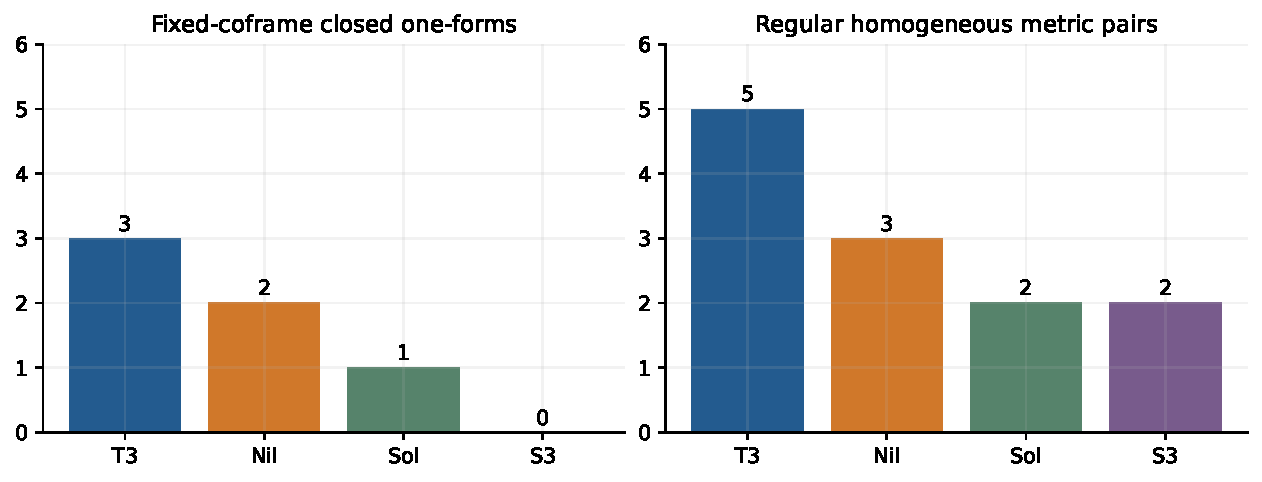
\includegraphics[width=.92\textwidth]{figures/fig01_distinct_counts.pdf}
\caption{Constant closed-one-form dimensions in the specified coframes and homogeneous pair counts on regular constraint strata. The static torus is not on the latter regular stratum.}\label{fig:fig01_distinct_counts}
\end{figure}

\subsection{The singular static torus}

The homogeneous mixed cone and exact family of Paper06, Section 5 and Appendix D, are placed here on the singular stratum of the Hamiltonian constraint $F$ \cite{paper6}. Sections 6--7 add nonzero Fourier components to this setting.

At $n=0$, $\pi=0$, $F$ is quadratic in momenta and $dF=0$. The quadratic action alone retains six metric pairs because its lapse equation vanishes. The second-order coefficient of the original nonlinear Hamiltonian constraint instead imposes the following condition, where $h$ is the first-order mean expansion and $\Sigma$ is tracefree.

\stepcounter{equation}\begin{equation}\tag{T-01}\label{eq:T-01}
K=\varepsilon(hI+\Sigma)+O(\varepsilon^2),\qquad \mathrm{tr}\Sigma=0,\qquad \mathrm{tr}(\Sigma^2)=6h^2.
\end{equation}

This cone is not a vector space. Its pure-scale slice requires $h=0$, while nontrivial simultaneous shape and volume directions exist. Replacing $p_q^2=0$ by $p_q=0$ changes its differential and gauge generator and is not an equivalent regularization.

\stepcounter{equation}\begin{equation}\tag{T-02}\label{eq:T-02}
\begin{aligned}g_{ii}(\tau,\varepsilon)&=q_0^2(1+3\varepsilon h\tau)^{2p_i},\quad p_i=\frac13+\frac{\sigma_i}{3h},\\ \sum_i\sigma_i&=0,\quad\sum_i\sigma_i^2=6h^2,\quad\sum_ip_i=\sum_ip_i^2=1.\end{aligned}
\end{equation}

For $h\ne0$, (T-02) is an exact vacuum solution on $1+3\varepsilon h\tau>0$, and its derivative in $\varepsilon$ realizes the cone direction. A general symmetric $\Sigma$ is recovered by a constant orthogonal matrix representation. If $h=0$, then $\Sigma=0$ and constant metric deformations remain. This explicit homogeneous construction is distinct from the theorem application for spatially dependent waves in Section 7.

The static flat-torus metric family is locally six-dimensional $\mathrm{SPD}(3)$, or five-dimensional at fixed volume, with residual discrete lattice identifications. Its pulled-back symplectic form vanishes because $\pi=0$; this does not make the whole family gauge.


The closed-one-form dimensions of Paper04 and frame comparisons of Paper06 serve as geometric data specifying the homogeneous truncation \cite{paper4,paper6}. Obtaining a reduced metric kernel from those dimensions would additionally require a map to perturbation fields compatible with constraints and gauge quotient. Appendix E collects the preceding geometric results in the present normalization.


\subsection{Linear rank exceptions at Taub points}

At the $S^3$ Taub background (BF-01), the homogeneous momentum rank is two and the full constraint rank is three. Axial $U(1)$ symmetry lowers these from the generic ranks three and four, giving a three-pair linear gauge quotient. This does not replace the two-pair regular-stratum result (H-04). Quadratic KID conditions remain, so the linear quotient is not identified with a smooth nonlinear physical phase space.

The $\ell,m$ tangent directions of the Taub family span one nondegenerate linear pair, while background time displacement is pure gauge. Further KID exceptions occur at low inhomogeneous labels and are counted with their representation multiplicities in Section 6.

%==============================================================================
% Section 6: Harmonic one-form realization of the zero kernel
%==============================================================================
\section{Harmonic one-form realisation of the zero kernel}
\label{sec:harmonic}

In this section we show how the scalar kernel of
Theorem~\ref{thm:rankdefect} is realised as a geometric object.  The claim is
within the left-invariant (representative) scope.

\subsection{Left-invariant harmonic one-forms and $\ker n$}
\label{sec:harmonic:lemma}

\begin{lemma}[Harmonic one-form $\Leftrightarrow\ker n$]
\label{lem:harmonic}
On the left-invariant coframe $\{\sigma^{i}\}$ of a Bianchi class-A geometry,
the space of left-invariant harmonic one-forms coincides with $\ker n$.
\end{lemma}

\begin{proof}
For a left-invariant one-form $\xi=\xi_{i}\,\sigma^{i}$ ($\xi_{i}$ constant), the
structure equations give
\begin{equation}
  \dd\xi = -\tfrac12\,\xi_{i}\,C^{i}{}_{jk}\,\sigma^{j}\wedge\sigma^{k},
\end{equation}
and since $C^{i}{}_{jk}=\epsilon_{jkl}n^{li}$ in class A,
\begin{equation}
  \dd\xi=0
  \quad\Longleftrightarrow\quad
  n\,\xi=0
  \quad\Longleftrightarrow\quad
  \xi\in\ker n.
\end{equation}
Moreover, for a left-invariant metric the co-closed condition
$\dd{\star}\xi=0$ is satisfied automatically by unimodularity (class A).  Hence
the harmonic one-forms are isomorphic to $\ker n$, of dimension $\dzero$.  On the
compact quotient they provide representatives of the de Rham $H^{1}$, realising
the geometric content of the coincidence with $b_{1}$
(Section~\ref{sec:rankdefect:b1})~\cite{ref41,ref42}.
\end{proof}

The agreement of the nullspaces of the exterior-derivative operator $d_{1}$ (on
left-invariant one-forms) and of $n$ is verifiable with
\code{script/scripts/paper07/harmonic_kernel_correspondence.py}.

\subsection{Map to the Hessian kernel}
\label{sec:harmonic:hessian}

Define the map from the scalar-axis perturbations $\beta_{a}$ to the
left-invariant one-form directions by
\begin{equation}
  \Phi:\ \beta_{a} \longmapsto \beta_{a}\,\sigma^{a}
\end{equation}
(no sum; Milnor frame).

\begin{proposition}[Hessian kernel $\leftrightarrow$ harmonic basis]
\label{prop:hessian}
The kernel of the scalar-axis Hessian of the reduced quadratic action is in
one-to-one correspondence with $\Phi(\ker n)$.  The map $\Phi$ preserves the
subspace (of dimension $\dzero$), not the axis names.
\end{proposition}

\begin{proof}[Proof sketch]
For $\beta\in\ker n$, Lemma~\ref{lem:harmonic} makes $\Phi(\beta)$ harmonic.  By
the activation rank of Section~\ref{sec:rankdefect:mechanism}, the $\beta$
direction does not activate a secondary constraint, and no kinetic pairing arises
in the scalar-axis Hessian.  Conversely, each direction of the Hessian kernel is
realised as a frame stretching along the basis $\xi^{(\alpha)}$ of $\ker n$
(Appendix~\ref{app:harmonic}).
\end{proof}

\subsection{Scope}
\label{sec:harmonic:scope}

This realisation is a correspondence at the left-invariant (homogeneous
representative) level, not a full Hodge-theoretic statement including the
inhomogeneous modes.  That no additional zero arises in the inhomogeneous sectors
is independently guaranteed by the non-contamination criterion of
Section~\ref{sec:spectral}.

%==============================================================================
% Section 7: Finite fate of the zero kernel
%==============================================================================
\section{Finite fate of the zero kernel}
\label{sec:finite}

After finding $\dzero$ non-propagating kernel directions at quadratic order, the
natural question is whether these are flat directions (moduli) under finite
deformation, or are blocked by walls at finite amplitude.  This section answers
that question \emph{within the finite Palatini branch / homogeneous
minisuperspace scope}.  \emph{This section is a supporting result and is not part
of Theorem~\ref{thm:rankdefect} (the quadratic theorem).}

\subsection{Classification: exact moduli versus curvature walls}
\label{sec:finite:classification}

For a finite deformation $\beta\mapsto\text{finite value}$ along a kernel
direction, we reconstruct a background-adapted static Palatini branch and verify
the finite expansion (symbolic, up to fourth order) of the reduced energy
density $\Delta(\beta)$.  The result is the following dichotomy:

\begin{itemize}
  \item \textbf{Exact modulus}: $\Delta(\beta)=0$ holds exactly at all orders of
        the expansion (a flat direction persisting under finite deformation).
  \item \textbf{Curvature wall}: $\Delta(\beta)$ develops a curvature-induced
        non-zero term (including a tadpole), and no stationary finite-deformation
        branch exists.
\end{itemize}

\paragraph{Key points at the level of formulas (finite Palatini branch /
homogeneous minisuperspace).}
\begin{itemize}
  \item \textbf{$\Tthree$}: the spatial scalar curvature vanishes identically.
        Hence $\Delta(\beta)\equiv0$ for any kernel direction (exact flat
        homogeneous branch).
  \item \textbf{$\Nilthree$ $\beta_{-}$}: along the tangent vector
        $(\tfrac12,-\tfrac12,0)$ in the Milnor frame, $\Delta(\beta_{-})=0$
        (residual $0$ up to fourth order; exact modulus).  The closed-form branch
        formula is in Appendix~\ref{app:finite:beta}.
  \item \textbf{$\Nilthree$ $\beta_{+}/u$}: along $(-\tfrac12,-\tfrac12,1)$ a
        curvature-induced linear term (tadpole) remains in the reduced energy; a
        curvature wall.
  \item \textbf{$\Solthree$ $\beta_{x}$}: along $(\tfrac13,-\tfrac16,-\tfrac16)$
        a non-zero term remains; no stationary branch (curvature wall).
\end{itemize}

\begin{table}[H]
\centering
\begingroup
\renewcommand{\arraystretch}{1.4}
\begin{tabularx}{\linewidth}{lrrrY}
\toprule
Topology & $\dzero$ & Exact moduli & Curvature wall & Remarks \\
\midrule
$\Tthree$ & 3 & 3 & 0 & exact flat homogeneous moduli \\
$\Nilthree$ & 2 & 1 ($\beta_{-}$) & 1 ($\beta_{+}/u$) &
$\beta_{-}$ exact modulus (residual $0$ to fourth order); $\beta_{+}$ wall with
tadpole \\
$\Solthree$ & 1 & 0 & 1 ($\beta_{x}$) & stationary branch absent \\
$\Sthree$ & 0 & 0 & 0 & $\dzero=0$ endpoint (not applicable) \\
\bottomrule
\end{tabularx}
\endgroup
\caption{Modulus/wall split (finite Palatini branch / homogeneous minisuperspace
scoped).}
\label{tab:modulus}
\end{table}

\begin{figure}[H]
  \centering
  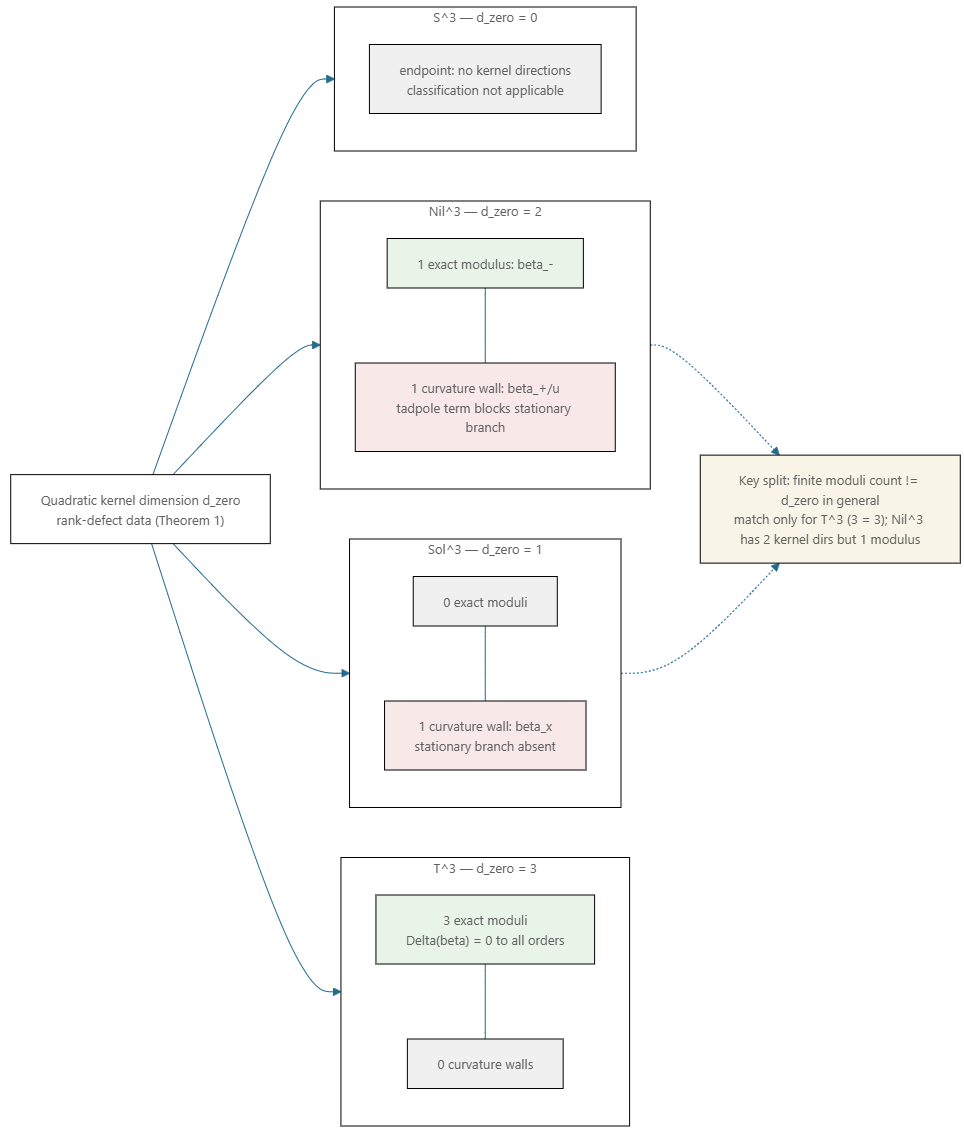
\includegraphics[width=0.95\textwidth]{figures/fig05_Modulus_wall-split.png}
  \caption{Modulus/wall split across the four topologies.  The correspondence
    between the quadratic kernel dimension $\dzero$ and the exact moduli /
    curvature walls on the finite Palatini branch is shown.  $\dzero$ is
    preserved as rank-defect data and does not in general equal the finite moduli
    count (they agree only for $\Tthree$).  \emph{Scope}: the wall checks are
    restricted to the finite Palatini branch / homogeneous minisuperspace; this
    is not a full nonlinear lift theorem.}
  \label{fig:modulus}
\end{figure}

\subsection{Minisuperspace DBR closure}
\label{sec:finite:minisuperspace}

The consistency of this classification was verified with the DBR closure of a
lever-complete homogeneous minisuperspace ansatz including the lapse, the
Hamiltonian constraint, and the DeWitt metric.  The results: (i) the closure
including the Hamiltonian constraint holds; (ii) the DeWitt norm of the
trace-free tangent directions is positive (minisuperspace no-ghost); and (iii)
the configuration degrees of freedom of the homogeneous anisotropy are $2$
(verification data in Appendix~\ref{app:finite}).

\subsection{Mandatory caveats}
\label{sec:finite:caveats}

\begin{itemize}
  \item \textbf{The finite moduli count is not in general equal to $\dzero$.}
        They agree only for $\Tthree$ (3$=$3); for $\Nilthree$ the exact modulus
        is $1$ against $\dzero=2$.  $\dzero$ is preserved as rank-defect data
        (the dimension of the quadratic kernel) and is a different quantity from
        the finite modulus count.
  \item \textbf{The wall checks are established within the finite Palatini
        branch}, and are not a full nonlinear lift theorem or mass theorem.  No
        extension to the time-dependent full DBR dynamics or to the inhomogeneous
        sector is made.
  \item \textbf{The minisuperspace no-ghost is not a full field-theory no-ghost}
        (the analysed scope of the latter is Section~\ref{sec:spectral}).
  \item The energy-density-expansion classification and the stationarity decision
        in the branch reconstruction are distinct checks, presented separately in
        Appendix~\ref{app:finite}.
\end{itemize}

\subsection{Torsion non-contamination (corollary)}
\label{sec:finite:torsion}

The torsion modes (EH/AX/VT/MX) do not change this modulus/wall split.  This is
a corollary of the triviality of the torsion auxiliary shell (not an independent
dynamical check); its precise statement is in Section~\ref{sec:torsion}.

%==============================================================================
% Section 8: Torsion/Nieh-Yan sector robustness
%==============================================================================
\section{Torsion/Nieh--Yan sector robustness}
\label{sec:torsion}

Although the action contains the NY term and torsion, the theorem and robustness
checks so far have not referred to torsion.  In this section we examine the
effect of the torsion sector on the preceding results.  The claim is confined to
a single point: \emph{the torsion sector affects none of the theorem hierarchy of
this paper (quadratic / $k>0$ spectral completion / finite deformation).}  The
physics of torsion itself (boundary charge, localisation, etc.) is outside the
scope of this paper.

\subsection{Known/new boundary}
\label{sec:torsion:boundary}

That the NY term is topological in the canonical analysis and does not change the
classical dynamics is known~\cite{ref33,ref34,ref35}.  The content of this
section is not a restatement of that generality but an \emph{exact demonstration
in the reduced system}: (i) the reduced action is exactly at most quadratic in
the torsion ansatz scalars; (ii) under field promotion no derivative coupling
arises in the inspected criterion; and (iii) the finite-deformation
classification is invariant.

\subsection{(i) Exact auxiliary shell}
\label{sec:torsion:shell}

The reduced torsion Lagrangian of the NY-MAIN route can be organised as an
auxiliary shell in the form
\begin{equation}
  \Laux
  = a_{\eta}\,\eta^{2} + a_{V}\,V^{2} + b_{V}\,\dot{\vol}\,V
    + \text{(boundary total-derivative)},
\end{equation}
(the coefficients $a_{\eta},a_{V},b_{V}$ are topology/mode dependent but
algebraic in $\eta,V$).  By a polynomial-degree verification (symbolic up to
degree 4, residual zero), it is \emph{exactly at most quadratic} in $(\eta,V)$.

\paragraph{Algebraic proof (shell condition).}
The Euler--Lagrange equations are
\begin{equation}
  \frac{\partial\Laux}{\partial\eta}=2a_{\eta}\,\eta=0,\qquad
  \frac{\partial\Laux}{\partial V}=2a_{V}\,V + b_{V}\,\dot{\vol}=0.
\end{equation}
If $a_{\eta}\ne0$ then $\eta^{\ast}=0$.  The linear term
$b_{V}\,\dot{\vol}\,V$ in $V$ can be separated as the boundary current
\begin{equation}
  2\,\frac{\dd}{\dd t}\!\left(\vol\cdot V\right),
\end{equation}
and the bulk equation gives $V^{\ast}=0$.  Hence
\begin{equation}
  \eta^{\ast}=0,\qquad V^{\ast}=0
\end{equation}
is an \emph{exact auxiliary shell}, not an approximation
(Appendix~\ref{app:torsion}).

\subsection{(ii) Field promotion does not generate kinetic terms}
\label{sec:torsion:promotion}

Decompose the connection as $\Gamma=\Gamma_{\mathrm{LC}}+K(\eta,V)$, with
\begin{equation}
  R[\Gamma]=\dd\Gamma+\Gamma\wedge\Gamma,\qquad
  K=K(\eta,V)\ \text{(algebraic in the $\AX/\VT/\MX$ ansatz scalars)}.
\end{equation}
If $K$ is algebraic in $\eta,V$ then $dK$ is first order in the field
derivatives, and the quadratic derivative couplings
$(\dot\eta^{2},\dot V^{2},(\nabla\eta)^{2},(\nabla V)^{2})$ in the scalar
contraction of $\Delta R$ cancel structurally (a native-action-gate statement;
not a full torsion field theory).

Promoting the scalars to fields $\eta(x),V(x)$, we inspected the above over all
cells of four topologies $\times$ $\AX/\VT/\MX$.  The results:

\begin{itemize}
  \item No quadratic derivative coupling appears at all.  Even a linear spatial
        gradient is absent.
  \item What appears is only a boundary-type time-linear current: $2\,\vol\cdot\dot V$
        on the EC side and $6\,\vol^{2/3}\,\dot\eta$ on the NY side.
  \item At the level of the Riemann components individual derivative terms fire,
        but they cancel under the scalar contraction, as confirmed by a
        component computation.
  \item The classification procedure is validated by positive-detector
        controls in the native-action gate that the witness checks before
        reporting the cells above: a free-scalar toy run through the same
        classifier recovers the expected positive time-kinetic and negative
        spatial-gradient coefficients (alongside ghost, wrong-sign, and
        linear-current toys), so a genuine kinetic term would be detected
        (\code{script/scripts/paper07/torsion_auxiliary_field_promotion_witness.py};
        no claim about a full 24-component torsion field theory).
\end{itemize}

\subsection{(iii) Finite fate is unchanged}
\label{sec:torsion:finite}

The modulus/wall split of Section~\ref{sec:finite} is invariant under all of the
torsion modes EH/AX/VT/MX (a corollary of $\Laux|_{\mathrm{shell}}=0$ on the
auxiliary shell).

\subsection{Conclusion and scope}
\label{sec:torsion:conclusion}

\begin{quote}
Within the NY-MAIN route and the $\AX/\VT/\MX$ torsion ansatz scalars, the
reduced torsion sector remains an exact auxiliary, and its promotion to fields
$\eta(x),V(x)$ generates no quadratic kinetic/gradient term in the inspected
native-action criterion.  Hence torsion/NY affects none of the DBR rank-defect
kernel (Section~\ref{sec:rankdefect}), the robustness from the $k>0$ spectral
completion (Section~\ref{sec:spectral}), or the finite homogeneous modulus/wall
split (Section~\ref{sec:finite}).
\end{quote}

\paragraph{Scope (explicit).}
The subject of this section is the $\AX/\VT/\MX$ ansatz scalars, not a
$(\partial T)^{2}$-absence theorem for a full 24-component torsion field theory.
The exact-degree-2 / exact-shell claim is restricted to the NY-MAIN route.  A
time-linear boundary current is not called a kinetic/propagating mode.  The
absence of NY bulk involvement is not claimed outside this scope.

\begin{table}[H]
\centering
\begingroup
\renewcommand{\arraystretch}{1.4}
\begin{tabularx}{\linewidth}{lLLl}
\toprule
Layer & Check & Result & Scope \\
\midrule
Quadratic & Polynomial-degree verification ($\eta,V$) &
exact degree-2; $\eta^{\ast}=V^{\ast}=0$ exact shell & NY-MAIN route \\
Finite & Invariance of the modulus/wall split &
invariant (corollary) & finite Palatini branch \\
Field-promoted & Derivative-coupling classification (4 topo.\ $\times$ AX/VT/MX) &
kinetic/gradient absent; boundary current only & inspected native-action
criterion \\
\bottomrule
\end{tabularx}
\endgroup
\caption{Hierarchy of the torsion robustness.}
\label{tab:torsion}
\end{table}

\section*{Acknowledgments}
The author acknowledges Claude Opus 4.8, Gemini 3.1 Pro, Grok 4.3, and GPT-5.5 Thinking via ChatGPT for assistance during preparation of the original manuscript in June 2026. For this revision, OpenAI Codex assisted with symbolic derivations, implementation, Japanese--English exposition and deterministic figure-generation code. The calculations and figures are reproducible from the supplied mathematical definitions and data. The author takes responsibility for the content and remaining errors.

This work was developed within the informal collaborative project \textbf{DPPU} (\textbf{D}onut-like topology, \textbf{P}lanck-scale compactness, \textbf{P}recession dynamics, \textbf{U}niverse).
\section*{Availability and contact}
The manuscript and supplement are available at \url{https://github.com/Muacca/DPPUv7-paper07}. The existing Zenodo record is \href{https://doi.org/10.5281/zenodo.20678646}{doi:10.5281/zenodo.20678646}; cite the edition and date of the artifact actually obtained. The supplement uses the MIT License. Contact: \href{mailto:muacca@dmwp.jp}{muacca@dmwp.jp}.

\appendix
\section{Fixed quotients and the convention dictionary}

On $T^3$, $x,y,z$ have period $2\pi$ and $\sigma=(dx,dy,dz)$. On Nil use $\sigma=(dx,dy,dz-xdy)$ with the following lattice generators.

\stepcounter{equation}\begin{equation}\tag{QA-01}\label{eq:QA-01}
(x,y,z)\sim(x+2\pi,y,z+2\pi y)\sim(x,y+2\pi,z)\sim(x,y,z+4\pi^2).
\end{equation}

Each generator preserves the coframe, and the fundamental volume is $(2\pi)^4$. The central Fourier factor is $e^{imz/(2\pi)}$, $m\in\mathbb Z$. The dual fields $X=\partial_x$, $Y=\partial_y+x\partial_z$, $Z=\partial_z$ give $-(X^2+Y^2+Z^2)$. The $m=0$ sector is the base torus; $m\ne0$ gives an oscillator with frequency $|m|/(2\pi)$ plus the central constant $m^2/(4\pi^2)$. Twisted periodicity gives $|m|$ independent states for each signed $m$.

For Sol take $\sigma=(dx,e^xdy,e^{-x}dz)$, $A=\left(\begin{smallmatrix}2&1\\1&1\end{smallmatrix}\right)$ and $\lambda=(3+\sqrt5)/2$. Choose a unit-area fiber lattice in eigenvector coordinates of $A$ and identify $(x,y,z)$ with $(x+\log\lambda,\lambda^{-1}y,\lambda z)$. Then $n_{23}=n_{32}=1$ and the reference volume is $\log\lambda$. Fiber Fourier covectors are grouped into dual-lattice orbits under $A$.

For simply connected $S^3=SU(2)$ use the unit round coframe satisfying $d\sigma^i=2\sigma^j\wedge\sigma^k$ cyclically. The metric $q^2\sum_i(\sigma^i)^2$ has sectional curvature $q^{-2}$, scalar curvature $6q^{-2}$ and volume $2\pi^2q^3$. A structure matrix defined with a negative structure equation changes sign when converted to the present convention. Axis changes must act consistently, including orientation, on metric, connection and torsion.

\stepcounter{equation}\begin{equation}\tag{QA-02}\label{eq:QA-02}
C^i{}_{jk}=\frac{a}{r}\epsilon_{ijk}\quad\Longrightarrow\quad q=\frac{2r}{|a|},\quad R=\frac{3a^2}{2r^2},\quad {\rm Vol}=\frac{16\pi^2r^3}{|a|^3}.
\end{equation}

Equation (QA-02) converts an orthonormal-frame structure magnitude $a/r$ to physical radius. Thus $a=1$ gives $q=2r$, $a=2$ gives $q=r$, and $a=4$ gives $q=r/2$. Curvature must not be converted while volume or wave numbers are left unchanged. The present calculation uses geometric torsion $T$ directly. The supplementary comparison guide gives implementation conversions.

\stepcounter{equation}\begin{equation}\tag{QA-03}\label{eq:QA-03}
\mathcal N=\frac14[abcd]T^e{}_{ab}T_{ecd}-\frac12[abcd]R_{abcd},\qquad[0123]=+1.
\end{equation}

The alternating symbol here is not the epsilon tensor with indices raised by the Lorentz metric. Both terms of complete NY use the same connection and agree with the exterior derivative in (A-01).


\subsection{Perturbation normalizations and symbols}

In the inhomogeneous calculations a common positive action factor is suppressed and integration uses fixed Haar measure. Symmetric metric components are ordered $(11,22,33,12,13,23)$, with conjugate momentum $\delta\pi^{ii}$ on the diagonal and $2\delta\pi^{ij}$ off the diagonal. Thus $J$ is the standard canonical matrix. A dagger includes complex conjugation and the formal spatial adjoint.

\stepcounter{equation}\begin{equation}\tag{QA-04}\label{eq:QA-04}
z=(h,p),\qquad J=\begin{pmatrix}0&I\\-I&0\end{pmatrix},\qquad
\Omega=-J,\qquad [X_i,X_j]=C^k{}_{ij}X_k.
\end{equation}

On Nil, $m$ is the central Fourier integer, $r$ a lattice copy, $n$ the oscillator index and $L$ the tensor grade. On $S^3$, $j,m,n$ are Wigner labels, independent of the background Taub parameter fixed to zero. On Sol, $x$ is the base coordinate and $\xi$ the unfolded real coordinate. The Nil period is also denoted $P_0=2\pi$ to distinguish it from the Gowdy field $P$; the LRS background value of $P$ in (NG-02) is $\bar P$ and $\zeta=e^{2\bar P}$. The Sol period is $L_{\rm Sol}=\log\lambda$, distinct from the Lagrangians $L_0$ and $L^{[2]}$ and from the Nil grade $L$.

%==============================================================================
% Appendix B: Native local action and DBR computational checks
%==============================================================================
\section{Native local action and DBR computational checks}
\label{app:native}

\subsection{Reduced action ingredients}
\label{app:native:action}

Under the homogeneous background ansatz (Section~\ref{sec:setup:perturbation}),
the first-order EC+NY action reduces to a finite-dimensional reduced Lagrangian.
The independent variables are the scale factors $q_{a}(t)$, the lapse $N(t)$, the
homogeneous connection components, and the torsion ansatz scalars $(\eta,V)$.
The perturbation analysis uses the quadratic action obtained by block-decomposing
this reduced system into scalar / spin-1 / spin-2 sectors.

\subsection{Symbolic Dirac--Bergmann engine}
\label{app:native:engine}

The constraint analysis was performed with a symbolic computation engine.  The
procedure follows the standard Dirac--Bergmann
algorithm~\cite{ref10,ref11,ref12}:
\begin{enumerate}
  \item Legendre transform and extraction of the primary constraints.
  \item Generation of the secondary constraints by the consistency conditions
        (iterated to closure).
  \item Classification of first/second class, and construction of the Dirac
        bracket for the second-class pairs.
  \item Presentation of the reduced spectrum by Routh-type elimination after
        closure (the DBR order).
\end{enumerate}

The decisions of the engine do not fix in advance the expected values of any
particular topology.  In the implementation, each topology local builder is
passed through the scalar-axis DBR closure, and the activation entry is read
from primary preservation, secondary generation, the constraint Poisson matrix
rank, and the first/second-class split.  The indeterminate-symbol relation
between the structure constants and the class-A matrix is checked separately as
a formal identity.  The physical role of that map as DBR activation is checked
by the axis-by-axis closure audit.

\paragraph{Correspondence with the proof skeleton of
Section~\ref{sec:rankdefect:mechanism}.}
Write $\Aop_{\rm DBR}$ for the secondary activation map for the scalar-axis
perturbations $\bm{\beta}\in\mathbb{R}^{3}$.  In the class-A Milnor frame, the
formal structure-map identity gives
\begin{equation}
  \Aop_{\rm form} = n .
\end{equation}
This identity is a notation and structure-map check; it is not used as a
substitute for DBR closure.  The witness
\code{rank_defect_activation_witness.py} calls the bundled DBR
constraint-closure engine (\code{dppu.dirac}) and computes the entries of
$\Aop_{\rm DBR}$ from DBR closure for the four topologies and three scalar
axes.  The resulting engine-derived activation matrix satisfies
$\rank(\Aop_{\rm DBR})=\rank(n)$ and
$\dim\ker(\Aop_{\rm DBR})=\dzero$.

\subsection{Rank verification conventions}
\label{app:native:rank}

For the rank decisions of the constraint matrices and the kinetic Hessians we
impose the following redundancies:
\begin{itemize}
  \item \textbf{Two routes}: agreement of the symbolic rank and the numerical
        rank is required.
  \item \textbf{Two generic points}: the numerical rank is evaluated at two
        generic background points, and agreement is required (excluding an
        accidental single-point degeneracy).
  \item \textbf{Mod-$p$ check}: for large symbolic matrices, a rank computation
        at a prime modulus is used in parallel to exclude a spurious rank from
        cancellation/round-off.
\end{itemize}

\subsection{Frame-invariance check protocol}
\label{app:native:frame}

The frame invariance of Section~\ref{sec:rankdefect:frame} is based first on the
analytic argument that $\rank(n)$ and $\dim\ker n$ are preserved under the
congruence $n\mapsto RnR^{\mathsf{T}}$.  The numerical verification reinforces it
by two routes: (a) random SO(3) rotations ($\dim\ker n$ preserved in all 20
rotations), and (b) reconstruction of $n$ from the rotated structure constants
(tensor transformation) and recomputation of the kernel dimension.  The script
\code{rank_defect_activation_witness.py} also confirms
$\rank(RnR^{\mathsf{T}})=\rank(n)$ for rational orthogonal matrices $R$.

\subsection{Comparison procedure under a single protocol}
\label{app:native:protocol}

The comparison of the four topologies was carried out under one and the same
engine, the same sector decomposition, and the same rank-verification conventions.
$\Sthree$ doubles as a cross-check of the method, passing the null check of the
scalar-axis projection (all axes zero for the isotropic $\Sthree$).

\subsection{Reproducibility notes}
\label{app:native:repro}

The main formulas and decisions in the paper are reproducible by the independent
witness scripts under \code{script/scripts/paper07/}.

\begin{table}[H]
\centering
\begingroup
\renewcommand{\arraystretch}{1.3}
\centering
\resizebox{\linewidth}{!}{%
\begin{tabular}{ll}
\toprule
Witness & Corresponding sections \\
\midrule
\code{rank_defect_activation_witness.py} &
\S\ref{sec:rankdefect:mechanism}--\ref{sec:rankdefect:frame},
\ref{app:native:engine}--\ref{app:native:frame}; *1 \\
\code{spectral_completion_witness.py} &
\S\ref{sec:spectral}, \ref{app:spectral} \\
\code{torsion_auxiliary_field_promotion_witness.py} &
\S\ref{sec:torsion}, \ref{app:torsion} \\
\code{finite_fate_branch_witness.py} &
\S\ref{sec:finite}, \ref{app:finite} \\
\code{harmonic_kernel_correspondence.py} &
\S\ref{sec:harmonic}, \ref{app:harmonic} \\
\code{route_comparison_s3_branch_a_witness.py} &
\S\ref{sec:dbr:control}, \ref{app:route} \\
\code{s3_normalization_factor_witness.py} &
\S\ref{sec:setup:structure}, \ref{app:conventions:s3} \\
\bottomrule
\end{tabular}%
}
\endgroup
\caption{Independent witness scripts and the sections they reproduce. (*1: formal identity as notation
check, DBR closure audit as primary evidence)}
\label{tab:witness}
\end{table}

\section{Constraint ranks and route controls}

A constant symmetric $n$ can be diagonalized by $SO(3)$. The $A_k$ in (H-03) represent the adjoint structure algebra; the Jacobi identity yields the momentum Poisson algebra. Both $T$ and $P$ are invariant under this action, giving $\{J,F\}=0$. In the six coordinates and their conjugates these statements are directly checkable polynomial identities.

\stepcounter{equation}\begin{equation}\tag{CC-01}\label{eq:CC-01}
\begin{aligned}g&=\mathrm{diag}(1,2,3),\quad c=1,\quad M=\pi g,\\ M_{T^3}&=\mathrm{diag}(1,1,0),\quad M_{\rm Nil}=\sqrt3 I,\\ M_{\rm Sol}&=\frac{5\sqrt3}{3}I,\quad M_{S^3}=\mathrm{diag}(4\sqrt2,0,0).\end{aligned}
\end{equation}

All representatives satisfy $F=J=0$. For $T^3$ the minor is $\partial F/\partial p_{33}=-6$. For the others take the required initial rows of $(F,J_1,J_2,J_3)$ and columns of $(p_{11},p_{23},p_{13},p_{12})$. Their determinants are $9\sqrt3$, $50\sqrt3$, and $-64\sqrt2$ for Nil, Sol and $S^3$, respectively; the Sol value uses the diagonalized $n=\mathrm{diag}(0,1,-1)$. Thus the constraint Jacobian ranks are $1/3/4/4$.

The spans of the $A_k$ have dimensions $0/2/3/3$, bounding the ranks of $J$. Near the nonzero minors, these maximal ranks and the independence of $dF$ persist, defining the regular strata of (H-04). Counts are not extended uniformly to points where minors vanish, such as symmetry-enhanced configurations.

\subsection{Closure for quadratic actions}

\stepcounter{equation}\begin{equation}\tag{CC-02}\label{eq:CC-02}
M_{A b}=\{\Phi_A,\phi_b\},\quad u^AM_{Ab}=0\quad\Longrightarrow\quad u^A\{\Phi_A,H_c\}\simeq0.
\end{equation}

Here $\phi$ denotes the original primaries and $\Phi$ all independent constraints available at the current stage. Add only new independent linear constraints from the left nullspace of $M$, iterating until none remain. For constant-coefficient quadratic actions this linear-algebra procedure is exact. It is not used to replace nonlinear constraints by linear-coefficient ranks. If the final Poisson rank is $s$ and there are $m$ independent constraints, their first- and second-class counts are $m-s$ and $s$.

\begin{center}\small\begin{tabularx}{\textwidth}{@{}>{\raggedright\arraybackslash}X>{\raggedright\arraybackslash}X>{\raggedright\arraybackslash}X@{}}\toprule
Control & Connection: FC/SC/pairs & Eliminated: FC/SC/pairs\\\midrule
Complete torus quadratic & 1 / 4 / 1 & 1 / 0 / 1\\
Complete sphere quadratic & 0 / 8 / 0 & 0 / 4 / 0\\
\bottomrule\end{tabularx}\end{center}

For the eliminated sphere block, $H=-p_u^2/24-6\ell u$ and $p_\ell=0$ give $u=0$, then $p_u=0$, then $\ell=0$. On the torus the lapse primary is first class and the quadratic action retains a scalar pair. Section 5 treats the condition from the original nonlinear constraint.


\subsection{Scalar controls from the complete action}

Set $c=1$, $n=2kI$ and write the independent scalar connection as $\omega^0{}_i=b e^i$, $\omega^j{}_k=a e^i$ cyclically. Here $k=0$ is the torus and $k=1$ the round-sphere reference.

\stepcounter{equation}\begin{equation}\tag{D-02}\label{eq:D-02}
L_{\rm P}=6Nq^3b^2-12q^2\dot q\,b+12kNq^2a-6Nq^3a^2,\quad a=k/q,\quad b=\dot q/(Nq).
\end{equation}

\stepcounter{equation}\begin{equation}\tag{D-03}\label{eq:D-03}
\begin{aligned}L_{\rm met}&=6k^2Nq-6q\dot q^2/N,\\ q&=1+\varepsilon u,\quad N=1+\varepsilon\ell,\quad a=k+\varepsilon A,\quad b=\varepsilon B,\\ L^{[1]}&=6k^2(\ell+u),\\ L_{\rm P}^{[2]}&=-6A^2-12kAu+6B^2-12B\dot u+6k^2\ell u-6k^2u^2,\\ L_{\rm met}^{[2]}&=-6\dot u^2+6k^2\ell u.\end{aligned}
\end{equation}

Substitution of the quadratic connection equations $A=-ku$, $B=\dot u$ gives the same metric action. The sphere has a nonzero first variation; the zero-pair agreement is an off-shell algebraic control. The torus quadratic scalar action retains one pair, while the original lapse equation requires $\dot u^2=0$, the pure-scale section of the cone in Section 5.


\subsection{Counts at symmetric Taub points and nonzero modes}

At the Taub point (BF-01), the homogeneous momentum and total ranks are two and three, leaving three pairs in the linear quotient. This is a different stratum from the regular representative (CC-01), with ranks three and four. Appendix G gives the $j=0,1$ KID exceptions and nonzero minors valid on the whole interval. The 40/34/10-configuration flat comparison in Section 4 counts one real Fourier quadrature, separately from the regular homogeneous count (H-04).

\section{Fourier action and integrated constraints}

\stepcounter{equation}\begin{equation}\tag{WD-01}\label{eq:WD-01}
\Gamma^{i(1)}{}_{jk}=\tfrac12(\partial_jh_{ik}+\partial_kh_{ij}-\partial_ih_{jk}),\quad R^{[1]}=\partial_i\partial_jh_{ij}-\partial^2h_{ii}.
\end{equation}

The second coefficient of the integrated $\sqrt g R$ Gamma--Gamma form gives the spatial term of (W-01). The first lapse perturbation multiplies $R^{[1]}$. With the wavevector along $z$, $R^{[1]}=k^2(h_{11}+h_{22})$; the shift enters through $v$, retaining all constraints. The momentum equations are proportional to $p_{13}=p_{23}=p_{33}=0$ and the linear Hamiltonian condition to $h_{11}+h_{22}=0$. These four secondaries and four primaries mutually Poisson commute.

For $k\ne0$, quotienting gauge directions and taking $h_{11}=-h_{22}=A$, $h_{12}=B$ gives (W-02). For any nonzero lattice wavevector the same algebra holds in an orthonormal polarization basis. The basis rotation need not be a lattice automorphism: the original wavevector and polarization tensors are restored.

\stepcounter{equation}\begin{equation}\tag{WD-02}\label{eq:WD-02}
\begin{aligned}R+K^2-K_{ij}K^{ij}&=0,\qquad D_j(K^{ij}-g^{ij}K)=0,\\ K^{[1]}&=hI+\Sigma+\tfrac12\dot\gamma,\qquad\left\langle R^{[2]}\right\rangle=-\tfrac1{4q_0^2}\left\langle(\partial_a\gamma_{ij})^2\right\rangle.\end{aligned}
\end{equation}

Zero-mean TT fields have vanishing averaged cross terms with constant $h,\Sigma$. The linear curvature of the second-order metric correction integrates to zero as a divergence, and because the background $K$ vanishes, the second-order correction to $K$ does not enter the quadratic constraint linearly. The averaged Hamiltonian constraint is therefore $6h^2-\mathrm{tr}\Sigma^2-\langle\dot\gamma^2\rangle/4-\langle(\partial\gamma)^2\rangle/(4q_0^2)=0$.

\stepcounter{equation}\begin{equation}\tag{WD-03}\label{eq:WD-03}
\mathcal J[\xi]=\int_\Sigma\pi^{ij}\mathcal L_\xi g_{ij},\quad \xi=\partial_a:\qquad \mathcal J^{[2]}[\partial_a]\ \propto\ \left\langle\dot\gamma_{ij}\partial_a\gamma_{ij}\right\rangle.
\end{equation}

Because background $\pi=0$ and $g$ is constant, linear terms in the second-order fields vanish, leaving (WD-03). Cross terms with constant mean metric or shear integrate to zero by periodicity. This gives the three momentum conditions in (W-03). The homogeneous linear equations keep $h,\Sigma$ constant, while the wave equation and periodic integration conserve wave energy and momentum.

The integrated conditions are the compact linearization-stability conditions \cite{BrillDeser1973,ArmsMarsdenMoncrief1982}. Positive TT energy excludes pure-wave directions but permits mixed directions with volume velocity. We next state their sufficiency on the fixed flat torus and give explicit second-order corrections.


\subsection{Application of the known theorem on the fixed flat torus}

\stepcounter{equation}\begin{equation}\tag{WD-04}\label{eq:WD-04}
\partial_i\partial_j\nu-\delta_{ij}\Delta\nu=0,\qquad
\partial_iX_j+\partial_jX_i=0,\qquad
\det(\mathcal S_k^\dagger\mathcal S_k)=32(k^2)^5\quad(k\ne0).
\end{equation}

In units $q_0=1$, (WD-04) describes the adjoint kernel. Taking the trace and using periodicity makes $\nu$ constant; the periodic Killing equation makes $X$ constant. These exhaust the four KIDs. Coordinate-linear rotations and boosts do not descend to the fixed lattice. The last identity checks the combined four-column symbol at nonzero wavevector.

\stepcounter{equation}\begin{equation}\tag{WD-05}\label{eq:WD-05}
\begin{aligned}
\delta g&=C+2t(hI+\Sigma)+\gamma, &\delta\pi&=\Sigma-2hI+\tfrac12\dot\gamma,\\
\beta&=\mathrm{tr}(\delta\pi)=-6h,&\omega^{\rm TT}&=\Sigma+\tfrac12\dot\gamma,\\
\langle(\omega^{\rm TT})^2\rangle-\beta^2/6
+\tfrac14\langle(\partial\gamma)^2\rangle
&=\mathrm{tr}\Sigma^2-6h^2+\tfrac14\langle\dot\gamma^2+(\partial\gamma)^2\rangle.
\end{aligned}
\end{equation}

$C$ and $\Sigma$ are constant, $\Sigma$ is tracefree and $\gamma$ is mean-zero TT. Equation (WD-05) identifies the Hamiltonian cone, Eq. (3.5) of Arms--Marsden--Moncrief, with the energy condition in (W-03); their momentum cones, Eq. (3.1), agree with (WD-03). Their Section 3 treats exactly a flat $g_0$ with $\pi_0=0$, and their introduction includes the flat spacetime $T^3\times\mathbb R$ with four Killing fields. We apply their Theorem 3.3 (Section 3, p. 96) to smooth periodic data on a compact boundaryless CMC slice. Curves may be interpreted, conservatively, in $H^s\times H^{s-1}$ for integer $s\ge5$, without claiming minimal regularity. The four conditions then characterize tangents to exact constraint-data curves. Local Cauchy development and the LC lift give EC vacuum families \cite{ArmsMarsdenMoncrief1982}.

This concerns a local initial-value family on a common time interval, not a two-time boundary-value problem, all-time regularity or an exact family closed in a finite Fourier space. Higher-order corrections may contain new harmonics.

\subsection{Explicit second-order corrections and two-wave closure}

For the standing wave (W-04), expanding each exponent as $\epsilon A_1+\epsilon^2A_2$, and similarly for $B,P$, makes the first and second coefficients of all ten Ricci components vanish, for either sign of $h$. This is a local substitution check through second order, not an exact finite-amplitude solution.

\stepcounter{equation}\begin{equation}\tag{WD-06}\label{eq:WD-06}
\begin{aligned}
f&=a\cos x\cos t,\quad g=b\cos y\cos t,\quad h^2=(a^2+b^2)/24,\\
H_{\mu\nu}&=\mathrm{diag}(-6ht,\,2ht+g,\,2ht+f,\,2ht-f-g),\\
\mathcal K&=\{(0,0),(\pm1,0),(0,\pm1),(\pm2,0),(0,\pm2),(\pm1,\pm1)\}.
\end{aligned}
\end{equation}

\stepcounter{equation}\begin{equation}\tag{WD-07}\label{eq:WD-07}
\begin{aligned}
\ddot{\bar Q}_{\mu\nu,n}+|n|^2\bar Q_{\mu\nu,n}&=-2G^{[2]}_{\mu\nu,n}[H],\\
-\dot{\bar Q}_{0\nu}+\partial_i\bar Q_{i\nu}&=0,\\
\psi&=-\tfrac7{16}(a^2\cos2x+b^2\cos2y)-ab\cos x\cos y,\\
\Delta\psi&=-2G^{[2]}_{00}[H](0),\\
\bar Q_{ij}(0)&=\delta_{ij}\psi,\qquad \bar Q_{00}(0)=\bar Q_{0i}(0)=0,\\
\dot{\bar Q}_{ij}(0)=\dot{\bar Q}_{00}(0)&=0,\qquad \dot{\bar Q}_{0i}(0)=\partial_i\psi.
\end{aligned}
\end{equation}

Write $g=\eta+\epsilon H+\epsilon^2Q$, with bars denoting trace reversal by $\eta$. Source conservation and the initial conditions in (WD-07) preserve the second-order harmonic condition. Keeping all thirteen wavevectors, integration of the forced oscillators constructs $Q$ satisfying the local Einstein equations and reality through second order. The public \texttt{two\_waves.json} supplies the source and correction coefficients. Removing the zero wavevector does not give the same construction.

%==============================================================================
% Appendix E: Harmonic form and Hessian kernel realization
%==============================================================================
\section{Harmonic form and Hessian kernel realisation}
\label{app:harmonic}

This appendix collects the verification tables for the correspondence of
Section~\ref{sec:harmonic}.

\subsection{Lemma~\ref{lem:harmonic} and Proposition~\ref{prop:hessian}}
\label{app:harmonic:checks}

For Lemma~\ref{lem:harmonic} ($\mathrm{nullspace}(d_{1})=\ker n$) and
Proposition~\ref{prop:hessian} (the map $\Phi:\beta_{a}\mapsto\beta_{a}\sigma^{a}$
relating the Hessian kernel and the harmonic basis), we confirmed the following
for each topology:
\begin{enumerate}
  \item \textbf{Closed condition}: for a left-invariant one-form
        $\xi=\xi_{i}\sigma^{i}$, $\dd\xi=0\Leftrightarrow n\xi=0$, with agreement
        of the exterior-derivative matrix $d_{1}$ and $n$,
        $\mathrm{nullspace}(d_{1})=\mathrm{nullspace}(n)$.
  \item \textbf{Co-closed condition}: under class A (unimodular), a
        left-invariant one-form is automatically co-closed ($\dd\star\xi=0$).
  \item \textbf{Hessian kernel dimension}: the kernel dimension of the
        scalar-axis Hessian $=\dim\ker n$ (a subspace decision, not an axis-name
        decision).
  \item \textbf{Correspondence of $\Phi$}: one-to-one (up to a change of basis)
        between the basis of $\ker n$ and the Hessian kernel directions.
  \item \textbf{Dimension agreement}:
        $\dim\{\text{harmonic one-forms}\}=\dzero=b_{1}$ ($\Tthree$:3,
        $\Nilthree$:2, $\Solthree$:1, $\Sthree$:0).
\end{enumerate}

Reproduction:
\code{script/scripts/paper07/harmonic_kernel_correspondence.py}.

\subsection{Per-topology kernel directions (Milnor frame)}
\label{app:harmonic:directions}

\begin{table}[H]
\centering
\begingroup
\renewcommand{\arraystretch}{1.4}
\begin{tabularx}{\linewidth}{llLY}
\toprule
Topology & $n$ & Basis of $\ker n$ & Harmonic one-forms \\
\midrule
$\Tthree$ & $\mathrm{diag}(0,0,0)$ & $e_{1},e_{2},e_{3}$ &
$\sigma^{1},\sigma^{2},\sigma^{3}$ \\
$\Nilthree$ & $\mathrm{diag}(1,0,0)$ & $e_{2},e_{3}$ &
$\sigma^{2},\sigma^{3}$ (the fibre direction $\sigma^{1}$ is non-harmonic) \\
$\Solthree$ & $\mathrm{diag}(1,-1,0)$ & $e_{3}$ &
$\sigma^{3}$ (single singular axis) \\
$\Sthree$ & $\mathrm{diag}(1,1,1)$ & $\{0\}$ & none \\
\bottomrule
\end{tabularx}
\endgroup
\caption{Per-topology kernel directions and harmonic one-forms (Milnor frame).}
\label{tab:kernel_directions}
\end{table}

The axis names depend on the Milnor frame convention; only the dimension is
frame-invariant (Section~\ref{sec:rankdefect:frame}).

\subsection{Scope note}
\label{app:harmonic:scope}

This correspondence is a realisation at the left-invariant representative level.
The de Rham $H^{1}$ representativeness on the compact quotient relies on standard
theory~\cite{ref18}, and that no additional zero arises in the inhomogeneous
sectors is independently guaranteed by the non-contamination criterion of
Section~\ref{sec:spectral}.

\section{Vacuum backgrounds, fixed quotients and harmonic bases}

\subsection{Background construction and descent to the quotients}

The Nil background in (BF-01) is Tanimoto\textquotesingle s homogeneous vacuum solution with $b=1$, Kasner exponents $(2/3,2/3,-1/3)$ and literature time $u^3$. Sol is the twisted Gowdy solution $P=2x,Q=0,R=t$. The biaxial Taub background uses $\ell=1,m=0$ and the conversion $\sigma=-\omega/2$. Direct substitution gives zero for the full Ricci tensor, both ADM constraints and the metric/momentum evolution residuals at the stated lapse. Time reparametrization does not change the lattice \cite{Tanimoto2004,Rendall2012,BeyerHennig2012}.

\stepcounter{equation}\begin{equation}\tag{BF-02}\label{eq:BF-02}
\begin{aligned}
\pi_{\rm Nil}^{ij}&=\mathrm{diag}(-4/(9A),-4/(9A),-u^2),\\
\pi_{\rm Sol}^{ij}&=\mathrm{diag}(-1/F,-t-1/(4t),-t-1/(4t)),\\
\pi^{ij}&=\sqrt{\det G}\,(K^{ij}-G^{ij}K),\qquad K_{ij}=\dot G_{ij}/(2N).
\end{aligned}
\end{equation}

The three Nil deck generators preserve the coframe in (QA-01). The Sol gluing preserves $(e^xdy,e^{-x}dz)$, and the $S^3$ coframe is global. Consequently the time-only $G,N$ descend to the fixed quotients. Positivity on the closed intervals follows directly from (BF-01).

\subsection{Central-nonzero Nil basis and tensor grade}

\stepcounter{equation}\begin{equation}\tag{NF-01}\label{eq:NF-01}
\begin{aligned}
\mu&=m/P_0,\quad m\in\mathbb Z\setminus\{0\},\quad 0\le r<|m|,\quad P_0=2\pi,\\
\Phi_{m,r,n}&=\sqrt{P_0}\,e^{i\mu z}\sum_{k\in\mathbb Z}
 e^{i(r+km)y}f_n\!\left(x+\frac{r+km}{\mu}\right),\\
f_n(v)&=\frac{(|\mu|/\pi)^{1/4}}{\sqrt{2^nn!}}
 H_n(\sqrt{|\mu|}v)e^{-|\mu|v^2/2}.
\end{aligned}
\end{equation}

Use normalized measure $dx\,dy\,dz/P_0^4$. The lattice shift in $x$ reindexes the sum, and the $y,z$ periods give integer phases, so (NF-01) descends to the quotient. Distinct $r,m$ are orthogonal. Unfolding the sum of $x$ intervals to the real line reduces normalization to that of $f_n$.

\stepcounter{equation}\begin{equation}\tag{NF-02}\label{eq:NF-02}
\begin{aligned}
(X-iY)\Phi_n&=\sqrt{2\mu n}\,\Phi_{n-1},&
(X+iY)\Phi_n&=-\sqrt{2\mu(n+1)}\,\Phi_{n+1},&Z\Phi_n&=i\mu\Phi_n\quad(m>0),\\
\theta^\pm&=(\sigma^1\pm i\sigma^2)/\sqrt2,&\theta^0&=\sigma^3,& L&=n+\mathrm{sign}(m)s.
\end{aligned}
\end{equation}

The symmetric tensor basis is $\theta^+\theta^+$, $(\theta^+\theta^0+\theta^0\theta^+)/\sqrt2$, $(\theta^+\theta^-+\theta^-\theta^+)/\sqrt2$, $\theta^0\theta^0$ and the two negative-spin partners, with spins $2,1,0,0,-1,-2$. For $m>0$ only components with $n=L-s\ge0$ exist. The LRS background has spin zero; ladder moves and tensor-spin moves preserve $L$. Applying the same rule to metric, momentum, lapse, shift and Cartan tensors closes a finite block. Complex conjugation gives $m<0$, with $r\mapsto-r\bmod|m|$ and $s\mapsto-s$.

The spin is a local rotation grading, not an additional global rotation KID of the quotient. Non-LRS coefficients couple $n$ to $n\pm2$ and destroy this finite-grade closure; this does not exclude other non-LRS analyses. At $m=0$ the usual base Fourier basis applies.

\subsection{Fixed Sol lattice and unfolding}

\stepcounter{equation}\begin{equation}\tag{SF-01}\label{eq:SF-01}
\begin{aligned}
\varphi&=(1+\sqrt5)/2,\quad\lambda=\varphi^2,\quad L_{\rm Sol}=\log\lambda,\\
S&=\frac1{\sqrt{1+\varphi^2}}\begin{pmatrix}1&-\varphi\\\varphi&1\end{pmatrix},\quad
D=\mathrm{diag}(\lambda^{-1},\lambda),\quad SA=DS,\\
q&=2\pi S(n_1,n_2)^T=(k_0,l_0)^T,\qquad q_j=(D^T)^jq,\\
k_0l_0&=\frac{4\pi^2}{\sqrt5}(n_1^2-n_1n_2-n_2^2)\ne0\quad(n\ne0).
\end{aligned}
\end{equation}

The fiber lattice is $S\mathbb Z^2$ with area one. The integer quadratic form in (SF-01) cannot vanish for a nonzero integer pair, so every nonzero dual orbit has both fiber components. Continuous covectors on a fiber axis are not modes of this fixed quotient.

\stepcounter{equation}\begin{equation}\tag{SF-02}\label{eq:SF-02}
\begin{aligned}
U_qf&=\sqrt{L_{\rm Sol}}\sum_{j\in\mathbb Z}f(x+jL_{\rm Sol})
 e^{i(\lambda^{-j}k_0y+\lambda^jl_0z)},\\
D_1&=\partial_\xi,\quad D_2=iK,\quad D_3=iM,
\qquad K=k_0e^{-\xi},\quad M=l_0e^\xi,\\
\mathcal D&=\{f:e^{a|\xi|}\partial_\xi^bf\in L^2(\mathbb R) \text{for all integers }a,b\ge0\}.
\end{aligned}
\end{equation}

For normalized measure $dx\,dy\,dz/L_{\rm Sol}$, $U$ is an isometry from $L^2(\mathbb R)$ onto the orbit space, by deck reindexing and fiber orthogonality. All coefficients, derivatives and formal adjoints are treated on $\mathcal D$, with zero boundary terms. Smooth compactly supported functions and Hermite functions belong to this core. This does not specify a closed operator extension or prove wellposedness.

\stepcounter{equation}\begin{equation}\tag{SF-03}\label{eq:SF-03}
[D_1,D_2]=-D_2,\quad[D_1,D_3]=D_3,\quad
e^\xi\psi_0= e^{1/4}\sum_{n=0}^{\infty}\frac{\psi_n}{2^{n/2}\sqrt{n!}}.
\end{equation}

Every coefficient in (SF-03) is nonzero, so no finite Hermite truncation is exactly closed. The infinite orbit is closed under all tensor components, constraints, gauge and evolution. Its conjugate orbit completes a real field. Fiber-zero modes instead use periodic base Fourier functions and form a distinct sector.

\subsection{Wigner blocks and reality on the three-sphere}

\stepcounter{equation}\begin{equation}\tag{TF-01}\label{eq:TF-01}
\begin{aligned}
Y^j_{mn}&=\sqrt{2j+1}\,D^j_{mn},\quad d=2j+1,\quad
\overline{Y^j_{mn}}=(-1)^{m-n}Y^j_{-m,-n},\\
D_a&=2iJ_a,\quad[D_a,D_b]=-2\epsilon_{abc}D_c,\quad
\sum_aD_a^2=-4j(j+1)I.
\end{aligned}
\end{equation}

Normalize Haar measure by the volume. Expand each of the six metric coefficients in the background coframe over all right indices. The left index supplies multiplicity; a complete real block at fixed $j$ contains $d^2$ real scalar components. Tensor coefficients obey the corresponding conjugation condition in (TF-01). We classify only $j=0,1/2,1,3/2$ explicitly and use $j=3/2$ for complete reconstruction.

\section{Constraint operators, reduction and reconstruction}

\subsection{Common construction}

\stepcounter{equation}\begin{equation}\tag{RG-01}\label{eq:RG-01}
\begin{aligned}
\mathcal H[N]&=\int N\left[\frac{\pi^{ij}\pi_{ij}-\pi^2/2}{\sqrt g}-\sqrt g\,R\right],\\
\mathcal H[X]&=\int\pi^{ij}\mathcal L_Xg_{ij},\qquad
Cz=\delta(\mathcal H_\perp,\mathcal H_i),\qquad
H=\delta^2\mathcal H[N],\\
S^{[2]}&=\int dt\,[p^\dagger\dot h-\tfrac12z^\dagger Hz-\alpha^\dagger Cz].
\end{aligned}
\end{equation}

Complex sectors are paired with their conjugates to give a real action. The Hamiltonian row of $C$ includes the background lapse because its multiplier is $\delta N/N$. Vary (RG-01) in the fixed frame, retaining its structure constants in Lie and covariant derivatives. For example, $\delta\Gamma=G^{-1}(\nabla h+\nabla h-\nabla h)/2$ and $\delta\mathrm{Ric}=\nabla\delta\Gamma-\nabla\delta\Gamma$ generate the spatial Hessian. These formulas define the public matrices reproducibly.

\stepcounter{equation}\begin{equation}\tag{RG-02}\label{eq:RG-02}
\begin{aligned}
CJC^\dagger&=0,\quad \dot C+CJH=BC,\quad
CE=GE=0,\quad E^\dagger\Omega E=\Omega_r,\\
H_r&=E^\dagger HE-E^\dagger\Omega\dot E,\quad
\dot z=JHz+JC^\dagger\alpha,\\
\alpha&=-(GJC^\dagger)^{-1}(\dot GE+GJHE)y,\qquad z=Ey.
\end{aligned}
\end{equation}

Select independent constraint rows at constant rank and impose $G$. The time derivative of $E$ in (RG-02) is essential on an evolving background, even when its contribution vanishes in a particular gauge. An independent four-dimensional Einstein variation checks the reconstructed spatial equations and time components proportional to constraints. The public coefficients expand and check this derivation.

\subsection{Nonzero base modes on Nil}

\stepcounter{equation}\begin{equation}\tag{NG-01}\label{eq:NG-01}
\begin{aligned}
Gz=0:&\quad h_{12}=h_{13}=0,\quad h_{22}/A+h_{33}/B_0=0,
\quad2A\delta\pi^{11}+2\pi^{11}_0h_{11}=0,\\
P&=h_{33}/B_0,\quad Q=h_{23}/B_0,\quad B_0=16u^2/(9A),\\
\Pi_P&=-A\delta\pi^{22}+B_0\delta\pi^{33}
+(A\pi^{22}_0+B_0\pi^{33}_0)P,\\
\Pi_Q&=B_0p_{23}+2B_0\pi^{22}_0Q.
\end{aligned}
\end{equation}

\stepcounter{equation}\begin{equation}\tag{NG-02}\label{eq:NG-02}
\begin{aligned}
P_{uu}+u^{-1}P_u+9(k^2+2\zeta)P-18ik\zeta Q&=0,\\
Q_{uu}+(u^{-1}+2\bar P_u)Q_u+9k^2Q+18ikP&=0,\\
\bar P=\log\frac{4u}{3(1+u^4)},\quad \zeta=e^{2\bar P},\quad R=4u/3,&\qquad k\ne0.
\end{aligned}
\end{equation}

These expressions align the base wavevector with one axis; the corresponding polarization rotation is restored for a general integer base direction. The chosen constraint minor is $-128ik^3u^5(1+u^4)/9$ and the gauge minor is $256ik^3u/81$, nonzero throughout the interval. Substitution of (NG-01) in (RG-02) gives (N-01) and then (NG-02). Off-diagonal spatial terms mix the cosine and sine quadratures. The interval bound $k^2-2\zeta\ge1/9$ does not define a time-independent conserved energy.

\subsection{Central-nonzero Nil blocks}

Expand (RG-01) in the basis (NF-02), including only multipliers present at each grade. Solve selected independent momentum columns from the constraints and fix their conjugate metric columns by gauge. Every existing constraint row has full rank. With $b=\sqrt\mu>0$, explicit minors at $L=-1,0,1,2$ are as follows; $L=-2$ has no constraint row.

\stepcounter{equation}\begin{equation}\tag{NG-03}\label{eq:NG-03}
\begin{aligned}
M_{-1}&=2b(1+u^4),\qquad M_0=-256b^3u^5/9,\\
M_1&=-\frac{512b^3u^3[9b^2u^2(1+u^4)^2+12u^4+4]}{81(1+u^4)},\\
M_2&=-2048b^3u^5(1+u^4)/9.
\end{aligned}
\end{equation}

For general $L\ge2$ there are six metric components and four multipliers. Finite closure identifies an adjoint kernel with a KID in the same central-nonzero sector, whereas the only quotient KID is the central-zero field $Z$. Thus all four constraints are independent, leaving two complex pairs. This structural argument is distinct from explicit matrices at five grades. The lower-end reduction comes from absent $n<0$ components, not a KID rank defect.

\stepcounter{equation}\begin{equation}\tag{NG-04}\label{eq:NG-04}
H_{r,-2}=-2\begin{pmatrix}
\dfrac{81\mu^2A^2-144\mu u^2+64}{72uA^2}&\dfrac{2(u^4-1)}{uA}\\[4pt]
\dfrac{2(u^4-1)}{uA}&\dfrac{9A^2}{2u}
\end{pmatrix}.
\end{equation}

Equation (NG-04) gives the one-pair lowest endpoint explicitly. Its sign in a time-dependent gauge does not by itself classify ghosts or instability. At $L=2$ the reduction, gauge multipliers and all ten Einstein components were independently compared; this four-dimensional check is not claimed uniformly for every grade.

\subsection{Fiber-zero Gowdy sector on Sol}

\stepcounter{equation}\begin{equation}\tag{SG-01}\label{eq:SG-01}
\begin{aligned}
ds^2&=-N^2dt^2+e^{2a}(dx+\beta dt)^2
+R[e^P(dy+Qdz)^2+e^{-P}dz^2],\\
R&=t+\rho,\quad P=2x+p,\quad Q=e^{-2x}r,\quad e^{2a_0}=F,\quad k=2\pi n/L_{\rm Sol},\\
C_H&=\delta p_R+(t-1/(4t))\delta p_a
+(2-1/(2t^2)-2k^2)\rho+2tikp,\\
C_x&=-2ik\delta a+ik(-2t-1/(2t))\rho+2\delta p_P-ik\delta p_a.
\end{aligned}
\end{equation}

For $n\ne0$, the gauge $\rho=\delta p_a=0$ has determinant $-2ik$. Eliminating $\delta a=\delta p_P/(ik)$ and $\delta p_R=-2tikp$ gives (SO-01). The two equations are $\ddot p+t^{-1}\dot p+k^2p=0$ and $\ddot r+t^{-1}\dot r+(k^2+4)r=0$. The auxiliary metric variable obeys $\ell=4t\dot p/(ik)$ and $\dot\ell=4iktp$.

\subsection{Differential right inverse for a general nonzero Sol orbit}

The following are differential identities on the entire orbit, not inverses of a finite truncation. Transform $h,p$ by $U=\mathrm{diag}(1,1,1,i,i,1)$ and the constraint rows by $\mathrm{diag}(1,1,-i,-i)$ to obtain real coefficients. Primes denote $\xi$ derivatives. Write the momentum part of $C=(C_q,C_p)$ as $C_pp=r$.

\stepcounter{equation}\begin{equation}\tag{SG-02}\label{eq:SG-02}
\begin{aligned}
r_0&=A_0p_{11}+p_{22}+p_{33},\quad A_0=F(4t^2-1)/(2t),\\
r_1&=-2Fp'_{11}+2t(p_{22}-p_{33})+F(Kp_{12}+Mp_{13}),\\
r_2&=-t(p'_{12}+p_{12}+2Kp_{22}+Mp_{23}),\\
r_3&=-t(p'_{13}-p_{13}+2Mp_{33}+Kp_{23}).
\end{aligned}
\end{equation}

\stepcounter{equation}\begin{equation}\tag{SG-03}\label{eq:SG-03}
\begin{aligned}
f&=p_{11},\quad b=Kp_{12}-Mp_{13},\quad V=K^2+M^2,\quad d_0=2-FV/(2t),\\
a&=\frac{-b'-(K^2-M^2)r_0+A_0(K^2-M^2)f-Vr_1/(2t)-FVf'/t-Kr_2/t+Mr_3/t}{d_0},\\
p_{22}&=(r_0-A_0f)/2+r_1/(4t)+Ff'/(2t)-Fa/(4t),\\
p_{33}&=(r_0-A_0f)/2-r_1/(4t)-Ff'/(2t)+Fa/(4t),\\
p_{12}&=(a+b)/(2K),\quad p_{13}=(a-b)/(2M),\\
p_{23}&=(-r_2/t-p'_{12}-p_{12}-2Kp_{22})/M.
\end{aligned}
\end{equation}

Using (SF-01), $F/t\ge e$ and $V\ge2|k_0l_0|$ gives $d_0\le2-4\pi^2e/\sqrt5<0$ for every nonzero lattice orbit on $1\le t\le2$. Define $E_p$ by setting $r=0$, and $R_p$ by setting $f=b=0$. With $TQ=(Q_1,0,0,KQ_2,-MQ_2,0)$, one obtains the complete splitting below.

\stepcounter{equation}\begin{equation}\tag{SG-04}\label{eq:SG-04}
\begin{aligned}
C_pE_p&=0,\quad C_pR_p=I,\quad T^\dagger E_p=I,\quad T^\dagger R_p=0,\\
E_pT^\dagger+R_pC_p&=I,\qquad Gz=R_p^\dagger h=0,\\
E&=\begin{pmatrix}T&0\\-R_pC_qT&E_p\end{pmatrix},\quad
Q=E_p^\dagger h,\quad\Pi=(p_{11},Kp_{12}-Mp_{13}),\\
GJC^\dagger&=I,\quad GJG^\dagger=0,\quad E^\dagger\Omega E=\Omega_r.
\end{aligned}
\end{equation}

The gauge is equivalent to $h_{22}=h_{33}=h_{23}=0$ and $h_{12}/K+h_{13}/M=0$. Here $E^\dagger\Omega\dot E$ vanishes exactly, but $\dot E$ remains in reconstruction. If $R$ is the reconstruction discrepancy, constraint and gauge preservation give $CR=GR=0$, while the reduced equation gives $E^\dagger\Omega R=0$. The complete splitting (SG-04) places $R$ in the range of $E$; nondegeneracy of $\Omega_r$ gives $R=0$. This proof does not require brute-force cancellation of every expanded reconstruction entry.

\stepcounter{equation}\begin{equation}\tag{SG-05}\label{eq:SG-05}
H_r=\sum_{a=0}^4 A_a(t,\xi)\partial_\xi^a,
\qquad H_r^\dagger=H_r,\qquad\mathrm{rank}\,A_4=1,\qquad(J_rA_4)^2=0.
\end{equation}

The public supplement expands all coefficients in (SG-05) and checks the highest-order rank and nilpotence. These facts alone do not imply hyperbolicity or stability.

\subsection{Low-label ranks and reconstruction on the three-sphere}

Per fixed left index, the constraint ranks at $j=0,1/2,1,3/2$ are $3,8,11,16$. Rational polynomial root counts, endpoints and denominators certify nonzero minors throughout $\tau\in[1/4,1/2]$. Restoring left multiplicity and reality gives the complete-block counts in the text. At $j=0$ the two-form on the $\ell,m$ parameter variations is $\left(\begin{smallmatrix}0&-64\\64&0\end{smallmatrix}\right)$; time displacement is pure gauge.

\stepcounter{equation}\begin{equation}\tag{TG-01}\label{eq:TG-01}
\begin{aligned}
T_q&=\mathrm{diag}(1,1,1,i,1,i)\otimes\mathrm{diag}(1,\sqrt3,\sqrt3,1),\\
Gz=0:&\quad h_{11}=h_{22}=h_{33}=h_{13}=0\quad\text{for all right indices},\\
\det M&=\frac{2^{52}\tau^4(\tau-1)^4(\tau+1)^4
(\tau^4-6\tau^2+33)^2(3\tau^4+14\tau^2+3)^2}{81(1+\tau^2)^4}.
\end{aligned}
\end{equation}

Equation (TG-01) gives the constant basis transformation and the selected minor at $j=3/2$; momenta transform by the inverse adjoint. With $w=(1,\sqrt3,\sqrt3,1)$, the eight free pairs are $h_{12}/(iw),h_{23}/(iw)$ and $-iwp_{12},-iwp_{23}$. Constructing $E$ and the multipliers by (RG-02), independent four-dimensional variation gives $\delta G_{ij}=0$, $\delta G_{00}=-NC_H/(2\sqrt g)$ and $\delta G_{0i}=-NC_i/(2\sqrt g)$. Including all left indices gives 32 real pairs.

\subsection{KIDs and quadratic necessary conditions}

\stepcounter{equation}\begin{equation}\tag{KG-01}\label{eq:KG-01}
\int_\Sigma\left(|D\nu|^2+K_{ij}K^{ij}\nu^2\right)dV=0
\quad\Longrightarrow\quad\nu=0.
\end{equation}

The selected backgrounds are CMC with $K_{ij}K^{ij}>0$, so (KG-01) applies to the KID lapse. The remaining spatial Killing fields must descend to the fixed quotient: one central field $Z$ on Nil, none on Sol, and four from $SU(2)\times U(1)$ on Taub. The central-nonzero Nil charge is (K-01); the conjugate $-m$ contribution adds with the same sign. The condition is imposed on the sum over blocks and allows inter-block cancellation. At $m=0$, $Z$ acts trivially.

\stepcounter{equation}\begin{equation}\tag{KG-02}\label{eq:KG-02}
L_a=-D_a^T,\qquad B_3=I_6\otimes D_3+S_3\otimes I_d,\qquad
(S_3h)_{ij}=-C^l{}_{3i}h_{lj}-C^l{}_{3j}h_{il}.
\end{equation}

The three left charges on $S^3$ are $\mathrm{Re}\sum\bar p L_ah$, and the axial charge is $\mathrm{Re}\sum\bar p B_3h$. Both terms in (KG-02) are required: the right scalar derivative alone omits the coframe spin. These are quadratic necessary conditions from (K-02).

\stepcounter{equation}\begin{equation}\tag{KG-03}\label{eq:KG-03}
\begin{aligned}
\left\langle2\delta p_P+\varepsilon\left[\delta p_P p_x+\delta p_r(r_x-2r)\right]\right\rangle&=0,\\
\langle\delta p_P^{(1)}\rangle=0,\qquad
2\langle\delta p_P^{(2)}\rangle+\left\langle\delta p_P^{(1)}p_x+\delta p_r(r_x-2r)\right\rangle&=0.
\end{aligned}
\end{equation}

Periodic metric reconstruction in Sol Gowdy requires the $x$-mean $\langle\cdot\rangle$ of $\Pi_PP_x+\Pi_QQ_x$ to vanish, where $\Pi_P,\Pi_Q$ are the momenta of $P,Q$ in (SG-01). With $p,r$ and their momenta $\delta p_P,\delta p_r$ of order $\varepsilon$, this mean equals $\varepsilon$ times the first line of (KG-03). The second line expands $\delta p_P=\delta p_P^{(1)}+\varepsilon\delta p_P^{(2)}+O(\varepsilon^2)$ and fixes the homogeneous second-order correction by first-order fields. It is not a KID charge of a general orbit. On the three curved backgrounds neither vanishing charges nor absence of KIDs is used to conclude nonlinear lifting sufficiency.

\section{Finite-time examples and numerical comparisons on Sol}

\subsection{Initial data and checks for finite blocks}

For Sol Gowdy take $n=1$ and initialize at $t=1$ from $p=J_0(kt)$ and $r=J_0(\sqrt{k^2+4}\,t)/2$ and their derivatives. For Nil base modes use wavevector $(1,0)$, $P=\sqrt2p\cos x$, $Q=\sqrt2q\sin x$ and $(p,p_u,q,q_u)=(0.2,0.07,-0.1,0.03)$ at $u=1$. Initial Hamiltonian momenta are obtained from (N-01).

For central Nil take $m=1,r=0,L=2$, with $Q=0$, $\Pi=(0.03,-0.02)$ at $u=1$. For $S^3$, excite left $m=+3/2$ at $j=3/2$ with $Q=0$, first momentum $0.03$ and sixth momentum $-0.02$ among the eight entries, at $\tau=1/4$, and add its real-field conjugate at left $m=-3/2$. Other entries initially vanish; all right indices and reconstructed metric components are retained.

DOP853 runs compare relative tolerances $10^{-10}$ and $10^{-12}$, with absolute tolerance smaller by a factor of 100, at 201 times on each interval. The table reports maximum component differences for the finer run, not rigorous error bounds.

\begin{center}\small\begin{tabularx}{\textwidth}{@{}>{\raggedright\arraybackslash}X>{\raggedright\arraybackslash}X>{\raggedright\arraybackslash}X>{\raggedright\arraybackslash}X@{}}\toprule
Example & Independent comparison & Maximum difference & Constraint\\\midrule
Nil base & Second order / Hamilton & $1.13\times10^{-12}$ & $3.89\times10^{-16}$\\
Nil central & Reduced / full ADM & $7.30\times10^{-13}$ & $6.94\times10^{-17}$\\
Sol Gowdy & Numerical / Bessel & $2.61\times10^{-12}$ & Analytic reconstruction\\
$S^3$ Taub & Reduced / full ADM & $1.45\times10^{-13}$ & $2.22\times10^{-15}$\\
\bottomrule\end{tabularx}\end{center}

The central Nil charge and all four $S^3$ charges vanish for these initial data and remain zero to numerical precision. These comparisons support finite-time linear examples. These numerical comparisons do not construct an exact nonlinear family. Local integrability of the admissible Sol initial data follows independently from the theorem application (SL-01).

\subsection{Independent four-dimensional Lorenz system on Sol}

\stepcounter{equation}\begin{equation}\tag{SH-01}\label{eq:SH-01}
\begin{aligned}
\mathcal F_\nu&=\nabla^\mu h_{\mu\nu}-\tfrac12\nabla_\nu h^\mu{}_\mu,\\
\delta R_{\mu\nu}-\nabla_{(\mu}\mathcal F_{\nu)}&=0,\qquad
H_{tt}=H_{\xi\xi}+B_xH_\xi+B_tH_t+B_0H.
\end{aligned}
\end{equation}

Direct Ricci variation in the noncoordinate frame of $\mathrm{diag}(-F,F,t,t)$ gives (SH-01). We use the standard Lorenz hyperbolic reduction, without WKB or geometric-optics approximations \cite{Andersson2021}. The ten components are ordered $(00,01,02,03,11,22,33,12,13,23)$ with phases $(1,1,i,i,1,1,1,i,i,1)$ to make coefficients real.

\stepcounter{equation}\begin{equation}\tag{SH-02}\label{eq:SH-02}
\begin{aligned}
H_{00}(1)=H_{0i}(1)&=0,\quad (h,p)(1)=E(1)y(1),\\
\mathcal F(1)&=\dot{\mathcal F}(1)=0,\qquad
y=-J_rE^\dagger Jz,\quad (-J_rE^\dagger J)E=I,\\
(-J_rE^\dagger J)JC^\dagger&=0.
\end{aligned}
\end{equation}

Match the spatial $H,\dot H$ to the same constrained ADM initial data, and determine $\dot H_{00},\dot H_{0i}$ from the Lorenz condition. The independent wave equation and ADM constraints also give $\dot{\mathcal F}(1)=0$ exactly. The projection (SH-02) removes gauge directions before comparison with the reduced variables $y$ of Appendix G; raw metric components in different gauges are not equated. All $B$ matrices and initial maps are supplied in the public supplement, implementing (RG-01) and direct Ricci variation.

\stepcounter{equation}\begin{equation}\tag{SH-03}\label{eq:SH-03}
\begin{aligned}
(n_1,n_2)&=(1,0),\quad \xi_0=\tfrac12\log(k_0/l_0),\\
y_\alpha(1,\xi)&=8^{1/4}\sum_{n=0}^{31}c_{\alpha n}
 \psi_n(\sqrt8(\xi-\xi_0)),\qquad \alpha=1,\ldots,4.
\end{aligned}
\end{equation}

The 128 coefficients are fixed in \texttt{data/initial/sol\_profile.json}, with a checked hash. They define the common initial profile. The profile is fixed input and is not interpreted as a conserved physical mode or frequency. Here $\psi_n$ is the normalized Hermite function; neither the orbit nor the basis is changed with time.

\subsection{Fixed discretization and three convergence comparisons}

\stepcounter{equation}\begin{equation}\tag{SH-04}\label{eq:SH-04}
\xi_j=\xi_0-W+\frac{2Wj}{N+1},\quad j=1,\ldots,N,\qquad
H(t,\xi)=\sum_{n=1}^N a_n(t)\sin\frac{n\pi(\xi-\xi_0+W)}{2W}.
\end{equation}

Use the time-fixed sine basis (SH-04), homogeneous Dirichlet conditions at its endpoints and DST spatial derivatives. These boundary conditions do not guarantee constraint preservation. On $|\xi-\xi_0|\le4$, $1\le t\le2$, continuum characteristic speed one leaves a margin of $0.25$ for $W=5.25$. The nonlocal spectral truncation is separately checked by changing the window; continuum causality alone does not imply zero numerical boundary error.

\begin{center}\small\begin{tabularx}{\textwidth}{@{}>{\raggedright\arraybackslash}X>{\raggedright\arraybackslash}X>{\raggedright\arraybackslash}X@{}}\toprule
Comparison & Parameters & Maximum reduced $L^2$ difference\\\midrule
Space &  $N=1023\to1535$, $W=5.25$ & $3.2645\times10^{-8}$\\
Window & $W=5.25\to5.6875$, $N=1535\to1663$ & $2.7682\times10^{-10}$\\
Time & rtol $10^{-12}\to3\times10^{-14}$, $N=1535$ & $3.9359\times10^{-9}$\\
\bottomrule\end{tabularx}\end{center}

Spatial and window comparisons use relative tolerance $3\times10^{-14}$ and absolute tolerance $3\times10^{-16}$. The window comparison keeps the grid spacing fixed. Fields at 101 saved times are interpolated to the same 2048-point interior Gauss--Legendre quadrature. The relative tolerance approaches double precision; the table reports numerical comparisons for this implementation.

\begin{figure}[htbp]\centering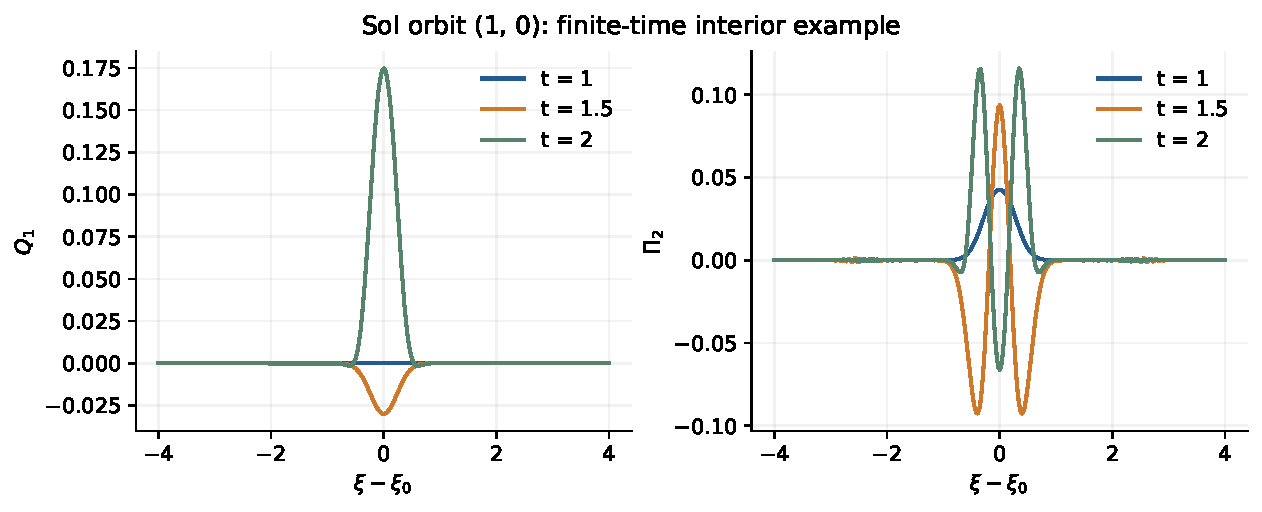
\includegraphics[width=.92\textwidth]{figures/fig05_sol_interior.pdf}
\caption{Reconstructed $Q_1$ and $\Pi_2$ on the interior from the same Sol initial profile. These are reduced variables in a finite-time example, not a gauge-independent metric observation or physical spectrum.}\label{fig:fig05_sol_interior}
\end{figure}

\subsection{Continuous-time residuals and unresolved scope}

\stepcounter{equation}\begin{equation}\tag{SH-05}\label{eq:SH-05}
\|v\|_I=\left(\int_{\xi_0-4}^{\xi_0+4}\sum_a|v_a|^2d\xi\right)^{1/2},\qquad
\rho_{\rm red}=\frac{\|\dot y-J_rH_ry\|_I}{\max(1,\|J_rH_ry\|_I)}.
\end{equation}

Analytically differentiate the actual accepted seventh-degree DOP853 dense polynomial at twenty times $t=1.025+0.05j$, $j=0,\ldots,19$, to obtain $H,\dot H,\ddot H$. These derivatives are substituted directly into the independent Ricci operator and the reduced fourth-order system (SG-05); $\ddot H$ is not replaced by the wave equation in (SH-01). Polynomial values are also compared directly with SciPy interpolation.

\begin{center}\small\begin{tabularx}{\textwidth}{@{}>{\raggedright\arraybackslash}X>{\raggedright\arraybackslash}X@{}}\toprule
Diagnostic & Maximum on the interior\\\midrule
Lorenz wave equation & $5.8631\times10^{-10}$\\
All ten Einstein components & $3.8255\times10^{-11}$\\
Lorenz constraint & $9.4853\times10^{-15}$\\
ADM constraint & $2.4617\times10^{-12}$\\
Reduced fourth-order $\rho_{\rm red}$ & $1.5388\times10^{-3}$\\
\bottomrule\end{tabularx}\end{center}

The first four rows are unnormalized $L^2$ norms of fixed-frame components; the last is the normalized residual (SH-05) of the reduced fourth-order system. Their magnitudes are not directly comparable error criteria. At the twenty times $\|J_rH_ry\|_I$ lies between $0.13$ and $2.7$, so the denominator in (SH-05) switches between absolute and relative normalization. The same residual is also evaluated on the four trajectories of the convergence comparisons at the 21 saved times $t=1,1.05,\ldots,2$, with $\ddot H$ given by the wave equation in (SH-01).

\begin{center}\small\begin{tabularx}{\textwidth}{@{}>{\raggedright\arraybackslash}X>{\raggedright\arraybackslash}X@{}}\toprule
Trajectory & Maximum $\rho_{\rm red}$ at the saved times\\\midrule
$N=1023$, $W=5.25$, rtol $3\times10^{-14}$ & $9.7624\times10^{-4}$\\
$N=1535$, $W=5.25$, rtol $3\times10^{-14}$ & $1.3726\times10^{-3}$\\
$N=1663$, $W=5.6875$, rtol $3\times10^{-14}$ & $9.6257\times10^{-4}$\\
$N=1535$, $W=5.25$, rtol $10^{-12}$ & $4.5461\times10^{-3}$\\
\bottomrule\end{tabularx}\end{center}

From $N=1023$ to $N=1535$ the residual does not decrease, and with the looser time tolerance it grows by a factor of about three. Convergence in the reduced fourth-order form is therefore not established. The independent Lorenz comparison supports a finite-time interior example. Whole-line error bounds, all-orbit or all-time stability and physical spectra remain unestablished. The continuous initial profile (SH-03) is covered by (SL-01), which does not certify exactness or convergence of the finite-window numerical trajectory.

\section{Revision note}

This version uses geometric torsion, constant complete NY, the physical spherical radius and fixed compact quotients. The epsilon-form action coefficient and spherical normalization of the first edition are corrected, and the vector divergence and endpoint data are treated within one action. Sections 2 and Appendices A--B specify the conventions; the changelog records the changes between editions.

The identification of constant closed-one-form dimensions with physical scalar kernels, the common physical TT spectrum asserted for all four geometries, and the interpretation of the former DBR/RBD difference as a physical ordering preference are withdrawn. Primary preservation requires the multiplier term of (D-01), and quadratic comparisons require matching perturbative order. Geometric closed forms, finite paths and Laplacians are retained in the domains specified in Appendix E.

\stepcounter{equation}\begin{equation}\tag{D-04}\label{eq:D-04}
\begin{aligned}L_{\rm old}&=-8s\dot b+12b^2-12a^2-4as-12\ell a-4\ell s,\\ L_{\rm old,red}&=-\tfrac43\dot s^2+3\ell^2-2\ell s+\tfrac13s^2,\\ \ell&=s/3,\qquad H_{PP}=-3/8.\end{aligned}
\end{equation}

Equation (D-04) is the strictly quadratic trace block of the lowest sphere harmonic in the first edition. Connection elimination and complete primary preservation both give one pair and the same $H_{PP}$. Appendix C gives the scalar comparison derived from the complete action. The supplementary comparison guide supplies the legacy-variable embedding and its relation to the 26-variable block.

This version derives the regular constraint counts for all symmetric homogeneous metrics and the action reduction of nonzero torus modes, connecting the homogeneous cone of Paper06 to compact conditions with TT energy and translation charges; under the hypotheses of Appendix D these conditions are sufficient for local integrability by the Arms--Marsden--Moncrief theorem. It also reduces linear perturbations on selected Nil, Sol and Taub vacuum backgrounds, with quadratic KID conditions and finite-time examples (Appendices F--H). Geometric results used from Papers 03EC, 04 and 06 are attributed and collected in Appendix E. Assumptions and derivations are given in the paper and appendices, with supplement reproduction instructions in the README.

\begin{thebibliography}{99}\footnotesize\raggedright
\setlength{\itemsep}{1pt}\setlength{\parsep}{0pt}
\bibitem{paper1} Muacca. Geometry-Dependent Classification of Reduced Potentials in Einstein--Cartan Gravity. v3 (2026). \href{https://doi.org/10.5281/zenodo.18213677}{doi:10.5281/zenodo.18213677}.
\bibitem{paper2} Muacca. Curvature Identities and Restricted Potential Bounds in Einstein--Cartan--Nieh--Yan Minisuperspace with Irreducible EC-Weyl Corrections. v2 (2026). \href{https://doi.org/10.5281/zenodo.18815498}{doi:10.5281/zenodo.18815498}.
\bibitem{paper3} Muacca. Spin-0, Spin-1 and Spin-2 Deformations of $S^3\times S^1$ in Einstein--Cartan--Nieh--Yan Theory. v3 (2026). \href{https://doi.org/10.5281/zenodo.19144481}{doi:10.5281/zenodo.19144481}.
\bibitem{paper3ec} Muacca. Curvature Components and Restricted Torsion Variations in Einstein--Cartan Minisuperspace. v4 (2026). \href{https://doi.org/10.5281/zenodo.19425147}{doi:10.5281/zenodo.19425147}.
\bibitem{paper4} Muacca. Kaluza--Klein Quadratic Forms and Torsion Boundary Data on Four Compact Geometries. v2 (2026). \href{https://doi.org/10.5281/zenodo.19775695}{doi:10.5281/zenodo.19775695}.
\bibitem{paper5} Muacca. Lorentzian Einstein--Cartan Reduction: Boundary Terms, Curvature Identities, and Homogeneous Variations. v2 (2026). \href{https://doi.org/10.5281/zenodo.20084722}{doi:10.5281/zenodo.20084722}.
\bibitem{paper6} Muacca. Lorentzian Einstein--Cartan Reduction on Four Homogeneous Geometries: Curvature, Boundary Terms, and Reduced Orbits. v2 (2026). \href{https://github.com/Muacca/DPPUv7-paper06}{Repository}; \href{https://doi.org/10.5281/zenodo.20228881}{doi:10.5281/zenodo.20228881}.
\bibitem{Hehl1976} F. W. Hehl, P. von der Heyde, G. D. Kerlick and J. M. Nester. General relativity with spin and torsion: Foundations and prospects. Rev. Mod. Phys. \textbf{48}, 393--416 (1976). \href{https://doi.org/10.1103/RevModPhys.48.393}{doi:10.1103/RevModPhys.48.393}.
\bibitem{NiehYan1982} H. T. Nieh and M. L. Yan. An identity in Riemann--Cartan geometry. J. Math. Phys. \textbf{23}, 373--374 (1982). \href{https://doi.org/10.1063/1.525379}{doi:10.1063/1.525379}.
\bibitem{GH1977} G. W. Gibbons and S. W. Hawking. Action integrals and partition functions in quantum gravity. Phys. Rev. D \textbf{15}, 2752--2756 (1977). \href{https://doi.org/10.1103/PhysRevD.15.2752}{doi:10.1103/PhysRevD.15.2752}.
\bibitem{HH1996} S. W. Hawking and G. T. Horowitz. The gravitational Hamiltonian, action, entropy and surface terms. Class. Quantum Grav. \textbf{13}, 1487--1498 (1996). \href{https://doi.org/10.1088/0264-9381/13/6/017}{doi:10.1088/0264-9381/13/6/017}.
\bibitem{Dirac1964} P. A. M. Dirac. \emph{Lectures on Quantum Mechanics}. Belfer Graduate School of Science, Yeshiva University (1964).
\bibitem{Pons2010} J. M. Pons. Substituting fields within the action: Consistency issues and some applications. J. Math. Phys. \textbf{51}, 122903 (2010). \href{https://arxiv.org/abs/0909.4151}{arXiv:0909.4151}.
\bibitem{Milnor1976} J. Milnor. Curvatures of left invariant metrics on Lie groups. Advances in Mathematics \textbf{21}(3), 293--329 (1976). \href{https://doi.org/10.1016/S0001-8708(76)80002-3}{doi:10.1016/S0001-8708(76)80002-3}.
\bibitem{Torre2004} C. G. Torre. Cosmology, cohomology and compactification. Class. Quantum Grav. \textbf{21}, L73 (2004). \href{https://arxiv.org/abs/gr-qc/0402105}{arXiv:gr-qc/0402105}.
\bibitem{Kasner1921} E. Kasner. Geometrical Theorems on Einstein's Cosmological Equations. American Journal of Mathematics \textbf{43}(4), 217--221 (1921). \href{https://doi.org/10.2307/2370192}{doi:10.2307/2370192}.
\bibitem{BrillDeser1973} D. R. Brill and S. Deser. Instability of closed spaces in general relativity. Commun. Math. Phys. \textbf{32}(4), 291--304 (1973). \href{https://doi.org/10.1007/BF01645610}{doi:10.1007/BF01645610}.
\bibitem{ArmsMarsdenMoncrief1982} J. M. Arms, J. E. Marsden and V. Moncrief. The structure of the space of solutions of Einstein's equations II: Several Killing fields and the Einstein--Yang--Mills equations. Annals of Physics \textbf{144}(1), 81--106 (1982). \href{https://doi.org/10.1016/0003-4916(82)90105-1}{doi:10.1016/0003-4916(82)90105-1}.
\bibitem{FischerMarsdenMoncrief1980} A. E. Fischer, J. E. Marsden and V. Moncrief. The structure of the space of solutions of Einstein's equations. I. One Killing field. Ann. Inst. H. Poincare A \textbf{33}(2), 147--194 (1980). \href{https://www.numdam.org/item/AIHPA_1980__33_2_147_0/}{Original article}. Theorem 2.1 and Lemma 2.2, pp.~161--162; function spaces on p.~155.
\bibitem{HughesKatoMarsden1977} T. J. R. Hughes, T. Kato and J. E. Marsden. Well-posed quasi-linear second-order hyperbolic systems with applications to nonlinear elastodynamics and general relativity. Arch. Rational Mech. Anal. \textbf{63}, 273--294 (1977). \href{https://www.cds.caltech.edu/~marsden/bib/1977/02-HuKaMa1977/HuKaMa1977.pdf}{Original article}. Theorem III and Section 5.
\bibitem{Nomizu1954} K. Nomizu. On the cohomology of compact homogeneous spaces of nilpotent Lie groups. Ann. of Math. \textbf{59}, 531--538 (1954). \href{https://doi.org/10.2307/1969716}{doi:10.2307/1969716}.
\bibitem{Hattori1960} A. Hattori. Spectral sequence in the de Rham cohomology of fibre bundles. J. Fac. Sci. Univ. Tokyo Sect. I \textbf{8}, 289--331 (1960).
\bibitem{Allen1995} B. Allen. Maximally symmetric spin-two bitensors on $S^3$ and $H^3$. Phys. Rev. D \textbf{51}, 5491--5497 (1995). \href{https://arxiv.org/abs/gr-qc/9411023}{arXiv:gr-qc/9411023}.
\bibitem{Andriot2018} D. Andriot and D. Tsimpis. Laplacian spectrum on a nilmanifold, truncations and effective theories. JHEP \textbf{09} (2018) 096. \href{https://arxiv.org/abs/1806.05156}{arXiv:1806.05156}.
\bibitem{Bolsinov2006} A. V. Bolsinov, H. R. Dullin and A. P. Veselov. Spectra of Sol-manifolds: Arithmetic and quantum monodromy. Commun. Math. Phys. \textbf{264}, 583--611 (2006). \href{https://arxiv.org/abs/math-ph/0503046}{arXiv:math-ph/0503046}.
\bibitem{Tanimoto2004} M. Tanimoto. Harmonic Analysis of Linear Fields on the Nilgeometric Cosmological Model. J. Math. Phys. \textbf{45}, 4896--4919 (2004); erratum \textbf{46}, 019902 (2005). \href{https://arxiv.org/abs/gr-qc/0402058v2}{arXiv:gr-qc/0402058v2}.
\bibitem{Rendall2012} A. D. Rendall. Dynamics of solutions of the Einstein equations with twisted Gowdy symmetry. J. Geom. Phys. \textbf{62}(3), 569--577 (2012). \href{https://doi.org/10.1016/j.geomphys.2011.04.016}{doi:10.1016/j.geomphys.2011.04.016}; \href{https://arxiv.org/abs/1011.2317v1}{arXiv:1011.2317v1}.
\bibitem{BeyerHennig2012} F. Beyer and J. Hennig. Smooth Gowdy symmetric generalized Taub--NUT solutions. Class. Quantum Grav. \textbf{29}, 245017 (2012). \href{https://arxiv.org/abs/1106.2377v2}{arXiv:1106.2377v2}.
\bibitem{Andersson2021} L. Andersson, J. Joudioux, M. A. Oancea and A. Raj. Propagation of polarized gravitational waves. Phys. Rev. D \textbf{103}, 044053 (2021). \href{https://arxiv.org/abs/2012.08363}{arXiv:2012.08363}.
\end{thebibliography}\end{document}
